\documentclass[twoside]{book}

% Packages required by doxygen
\usepackage{fixltx2e}
\usepackage{calc}
\usepackage{doxygen}
\usepackage[export]{adjustbox} % also loads graphicx
\usepackage{graphicx}
\usepackage[utf8]{inputenc}
\usepackage{makeidx}
\usepackage{multicol}
\usepackage{multirow}
\PassOptionsToPackage{warn}{textcomp}
\usepackage{textcomp}
\usepackage[nointegrals]{wasysym}
\usepackage[table]{xcolor}

% Font selection
\usepackage[T1]{fontenc}
\usepackage[scaled=.90]{helvet}
\usepackage{courier}
\usepackage{amssymb}
\usepackage{sectsty}
\renewcommand{\familydefault}{\sfdefault}
\allsectionsfont{%
  \fontseries{bc}\selectfont%
  \color{darkgray}%
}
\renewcommand{\DoxyLabelFont}{%
  \fontseries{bc}\selectfont%
  \color{darkgray}%
}
\newcommand{\+}{\discretionary{\mbox{\scriptsize$\hookleftarrow$}}{}{}}

% Page & text layout
\usepackage{geometry}
\geometry{%
  a4paper,%
  top=2.5cm,%
  bottom=2.5cm,%
  left=2.5cm,%
  right=2.5cm%
}
\tolerance=750
\hfuzz=15pt
\hbadness=750
\setlength{\emergencystretch}{15pt}
\setlength{\parindent}{0cm}
\setlength{\parskip}{3ex plus 2ex minus 2ex}
\makeatletter
\renewcommand{\paragraph}{%
  \@startsection{paragraph}{4}{0ex}{-1.0ex}{1.0ex}{%
    \normalfont\normalsize\bfseries\SS@parafont%
  }%
}
\renewcommand{\subparagraph}{%
  \@startsection{subparagraph}{5}{0ex}{-1.0ex}{1.0ex}{%
    \normalfont\normalsize\bfseries\SS@subparafont%
  }%
}
\makeatother

% Headers & footers
\usepackage{fancyhdr}
\pagestyle{fancyplain}
\fancyhead[LE]{\fancyplain{}{\bfseries\thepage}}
\fancyhead[CE]{\fancyplain{}{}}
\fancyhead[RE]{\fancyplain{}{\bfseries\leftmark}}
\fancyhead[LO]{\fancyplain{}{\bfseries\rightmark}}
\fancyhead[CO]{\fancyplain{}{}}
\fancyhead[RO]{\fancyplain{}{\bfseries\thepage}}
\fancyfoot[LE]{\fancyplain{}{}}
\fancyfoot[CE]{\fancyplain{}{}}
\fancyfoot[RE]{\fancyplain{}{\bfseries\scriptsize Generated by Doxygen }}
\fancyfoot[LO]{\fancyplain{}{\bfseries\scriptsize Generated by Doxygen }}
\fancyfoot[CO]{\fancyplain{}{}}
\fancyfoot[RO]{\fancyplain{}{}}
\renewcommand{\footrulewidth}{0.4pt}
\renewcommand{\chaptermark}[1]{%
  \markboth{#1}{}%
}
\renewcommand{\sectionmark}[1]{%
  \markright{\thesection\ #1}%
}

% Indices & bibliography
\usepackage{natbib}
\usepackage[titles]{tocloft}
\setcounter{tocdepth}{3}
\setcounter{secnumdepth}{5}
\makeindex

% Hyperlinks (required, but should be loaded last)
\usepackage{ifpdf}
\ifpdf
  \usepackage[pdftex,pagebackref=true]{hyperref}
\else
  \usepackage[ps2pdf,pagebackref=true]{hyperref}
\fi
\hypersetup{%
  colorlinks=true,%
  linkcolor=blue,%
  citecolor=blue,%
  unicode%
}

% Custom commands
\newcommand{\clearemptydoublepage}{%
  \newpage{\pagestyle{empty}\cleardoublepage}%
}

\usepackage{caption}
\captionsetup{labelsep=space,justification=centering,font={bf},singlelinecheck=off,skip=4pt,position=top}

%===== C O N T E N T S =====

\begin{document}

% Titlepage & ToC
\hypersetup{pageanchor=false,
             bookmarksnumbered=true,
             pdfencoding=unicode
            }
\pagenumbering{roman}
\begin{titlepage}
\vspace*{7cm}
\begin{center}%
{\Large Memory Manager }\\
\vspace*{1cm}
{\large Generated by Doxygen 1.8.11}\\
\end{center}
\end{titlepage}
\clearemptydoublepage
\tableofcontents
\clearemptydoublepage
\pagenumbering{arabic}
\hypersetup{pageanchor=true}

%--- Begin generated contents ---
\chapter{Class Index}
\section{Class List}
Here are the classes, structs, unions and interfaces with brief descriptions\+:\begin{DoxyCompactList}
\item\contentsline{section}{\hyperlink{classMemoryManager}{Memory\+Manager} \\*A memory management unit }{\pageref{classMemoryManager}}{}
\item\contentsline{section}{\hyperlink{structMemoryPairAddress__t}{Memory\+Pair\+Address\+\_\+t} }{\pageref{structMemoryPairAddress__t}}{}
\item\contentsline{section}{\hyperlink{classPageTable}{Page\+Table} \\*Page table holding page/frame pairs }{\pageref{classPageTable}}{}
\item\contentsline{section}{\hyperlink{classPhysicalMemory}{Physical\+Memory} \\*Imitates a physical memory }{\pageref{classPhysicalMemory}}{}
\end{DoxyCompactList}

\chapter{File Index}
\section{File List}
Here is a list of all files with brief descriptions\+:\begin{DoxyCompactList}
\item\contentsline{section}{src/\hyperlink{main_8cpp}{main.\+cpp} }{\pageref{main_8cpp}}{}
\item\contentsline{section}{src/\hyperlink{memory_8cpp}{memory.\+cpp} }{\pageref{memory_8cpp}}{}
\item\contentsline{section}{src/\hyperlink{memory_8h}{memory.\+h} }{\pageref{memory_8h}}{}
\end{DoxyCompactList}

\chapter{Class Documentation}
\hypertarget{classMemoryManager}{}\section{Memory\+Manager Class Reference}
\label{classMemoryManager}\index{Memory\+Manager@{Memory\+Manager}}


A memory management unit.  




{\ttfamily \#include $<$memory.\+h$>$}



Collaboration diagram for Memory\+Manager\+:
\nopagebreak
\begin{figure}[H]
\begin{center}
\leavevmode
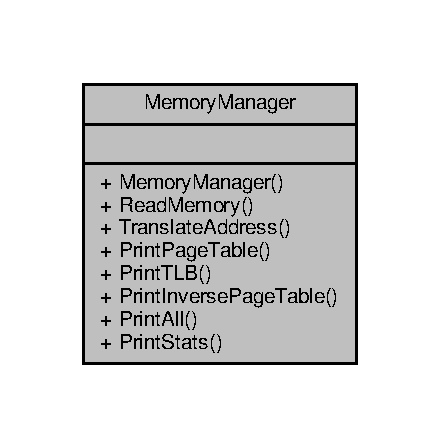
\includegraphics[width=211pt]{classMemoryManager__coll__graph}
\end{center}
\end{figure}
\subsection*{Public Member Functions}
\begin{DoxyCompactItemize}
\item 
\hyperlink{classMemoryManager_ae925e8ad4d8fe6f0565e9d5729f59593}{Memory\+Manager} ()
\begin{DoxyCompactList}\small\item\em Constructor. \end{DoxyCompactList}\item 
char \hyperlink{classMemoryManager_a4a716fc46ee321ebb25bd54bcc9d0524}{Read\+Memory} (int addr)
\begin{DoxyCompactList}\small\item\em Read a value from memory. \end{DoxyCompactList}\item 
int \hyperlink{classMemoryManager_a905ceff7ad39c05c2d965af613156547}{Translate\+Address} (int addr)
\begin{DoxyCompactList}\small\item\em Translate a virual address (P, d) to a physical address (f, d). Doesn\textquotesingle{}t implement any p. \end{DoxyCompactList}\item 
void \hyperlink{classMemoryManager_aa7437efdc1ebd09895d451e2c521857a}{Print\+Page\+Table} ()
\begin{DoxyCompactList}\small\item\em Print the page table. \end{DoxyCompactList}\item 
void \hyperlink{classMemoryManager_a4bc5f491976e5253bf00a07a71b55ef6}{Print\+T\+LB} ()
\begin{DoxyCompactList}\small\item\em Print the T\+LB. \end{DoxyCompactList}\item 
void \hyperlink{classMemoryManager_a231141529c907c50de129169f16bedf1}{Print\+Inverse\+Page\+Table} ()
\begin{DoxyCompactList}\small\item\em Print Inverse page table. \end{DoxyCompactList}\item 
void \hyperlink{classMemoryManager_ae7bbb5231788516ca34caca3d428b0ef}{Print\+All} ()
\begin{DoxyCompactList}\small\item\em Print T\+LB and Page Table. \end{DoxyCompactList}\item 
void \hyperlink{classMemoryManager_ad0c7c13901cb9c6844aebf6bf9238c47}{Print\+Stats} ()
\begin{DoxyCompactList}\small\item\em Print statistics for page faults and hit rate. \end{DoxyCompactList}\end{DoxyCompactItemize}


\subsection{Detailed Description}
A memory management unit. 

Definition at line \hyperlink{memory_8h_source_l00251}{251} of file \hyperlink{memory_8h_source}{memory.\+h}.



\subsection{Constructor \& Destructor Documentation}
\index{Memory\+Manager@{Memory\+Manager}!Memory\+Manager@{Memory\+Manager}}
\index{Memory\+Manager@{Memory\+Manager}!Memory\+Manager@{Memory\+Manager}}
\subsubsection[{\texorpdfstring{Memory\+Manager()}{MemoryManager()}}]{\setlength{\rightskip}{0pt plus 5cm}Memory\+Manager\+::\+Memory\+Manager (
\begin{DoxyParamCaption}
{}
\end{DoxyParamCaption}
)}\hypertarget{classMemoryManager_ae925e8ad4d8fe6f0565e9d5729f59593}{}\label{classMemoryManager_ae925e8ad4d8fe6f0565e9d5729f59593}


Constructor. 



Definition at line \hyperlink{memory_8cpp_source_l00291}{291} of file \hyperlink{memory_8cpp_source}{memory.\+cpp}.



\subsection{Member Function Documentation}
\index{Memory\+Manager@{Memory\+Manager}!Print\+All@{Print\+All}}
\index{Print\+All@{Print\+All}!Memory\+Manager@{Memory\+Manager}}
\subsubsection[{\texorpdfstring{Print\+All()}{PrintAll()}}]{\setlength{\rightskip}{0pt plus 5cm}void Memory\+Manager\+::\+Print\+All (
\begin{DoxyParamCaption}
{}
\end{DoxyParamCaption}
)}\hypertarget{classMemoryManager_ae7bbb5231788516ca34caca3d428b0ef}{}\label{classMemoryManager_ae7bbb5231788516ca34caca3d428b0ef}


Print T\+LB and Page Table. 



Definition at line \hyperlink{memory_8cpp_source_l00432}{432} of file \hyperlink{memory_8cpp_source}{memory.\+cpp}.

\index{Memory\+Manager@{Memory\+Manager}!Print\+Inverse\+Page\+Table@{Print\+Inverse\+Page\+Table}}
\index{Print\+Inverse\+Page\+Table@{Print\+Inverse\+Page\+Table}!Memory\+Manager@{Memory\+Manager}}
\subsubsection[{\texorpdfstring{Print\+Inverse\+Page\+Table()}{PrintInversePageTable()}}]{\setlength{\rightskip}{0pt plus 5cm}void Memory\+Manager\+::\+Print\+Inverse\+Page\+Table (
\begin{DoxyParamCaption}
{}
\end{DoxyParamCaption}
)}\hypertarget{classMemoryManager_a231141529c907c50de129169f16bedf1}{}\label{classMemoryManager_a231141529c907c50de129169f16bedf1}


Print Inverse page table. 



Definition at line \hyperlink{memory_8cpp_source_l00437}{437} of file \hyperlink{memory_8cpp_source}{memory.\+cpp}.

\index{Memory\+Manager@{Memory\+Manager}!Print\+Page\+Table@{Print\+Page\+Table}}
\index{Print\+Page\+Table@{Print\+Page\+Table}!Memory\+Manager@{Memory\+Manager}}
\subsubsection[{\texorpdfstring{Print\+Page\+Table()}{PrintPageTable()}}]{\setlength{\rightskip}{0pt plus 5cm}void Memory\+Manager\+::\+Print\+Page\+Table (
\begin{DoxyParamCaption}
{}
\end{DoxyParamCaption}
)}\hypertarget{classMemoryManager_aa7437efdc1ebd09895d451e2c521857a}{}\label{classMemoryManager_aa7437efdc1ebd09895d451e2c521857a}


Print the page table. 



Definition at line \hyperlink{memory_8cpp_source_l00424}{424} of file \hyperlink{memory_8cpp_source}{memory.\+cpp}.

\index{Memory\+Manager@{Memory\+Manager}!Print\+Stats@{Print\+Stats}}
\index{Print\+Stats@{Print\+Stats}!Memory\+Manager@{Memory\+Manager}}
\subsubsection[{\texorpdfstring{Print\+Stats()}{PrintStats()}}]{\setlength{\rightskip}{0pt plus 5cm}void Memory\+Manager\+::\+Print\+Stats (
\begin{DoxyParamCaption}
{}
\end{DoxyParamCaption}
)}\hypertarget{classMemoryManager_ad0c7c13901cb9c6844aebf6bf9238c47}{}\label{classMemoryManager_ad0c7c13901cb9c6844aebf6bf9238c47}


Print statistics for page faults and hit rate. 



Definition at line \hyperlink{memory_8cpp_source_l00441}{441} of file \hyperlink{memory_8cpp_source}{memory.\+cpp}.

\index{Memory\+Manager@{Memory\+Manager}!Print\+T\+LB@{Print\+T\+LB}}
\index{Print\+T\+LB@{Print\+T\+LB}!Memory\+Manager@{Memory\+Manager}}
\subsubsection[{\texorpdfstring{Print\+T\+L\+B()}{PrintTLB()}}]{\setlength{\rightskip}{0pt plus 5cm}void Memory\+Manager\+::\+Print\+T\+LB (
\begin{DoxyParamCaption}
{}
\end{DoxyParamCaption}
)}\hypertarget{classMemoryManager_a4bc5f491976e5253bf00a07a71b55ef6}{}\label{classMemoryManager_a4bc5f491976e5253bf00a07a71b55ef6}


Print the T\+LB. 



Definition at line \hyperlink{memory_8cpp_source_l00428}{428} of file \hyperlink{memory_8cpp_source}{memory.\+cpp}.

\index{Memory\+Manager@{Memory\+Manager}!Read\+Memory@{Read\+Memory}}
\index{Read\+Memory@{Read\+Memory}!Memory\+Manager@{Memory\+Manager}}
\subsubsection[{\texorpdfstring{Read\+Memory(int addr)}{ReadMemory(int addr)}}]{\setlength{\rightskip}{0pt plus 5cm}char Memory\+Manager\+::\+Read\+Memory (
\begin{DoxyParamCaption}
\item[{int}]{addr}
\end{DoxyParamCaption}
)}\hypertarget{classMemoryManager_a4a716fc46ee321ebb25bd54bcc9d0524}{}\label{classMemoryManager_a4a716fc46ee321ebb25bd54bcc9d0524}


Read a value from memory. 


\begin{DoxyParams}{Parameters}
{\em int} & Virtual address to read from. \\
\hline
\end{DoxyParams}

\begin{DoxyRetVals}{Return values}
{\em char} & value from mem\mbox{[}addr\mbox{]} \\
\hline
\end{DoxyRetVals}


Definition at line \hyperlink{memory_8cpp_source_l00299}{299} of file \hyperlink{memory_8cpp_source}{memory.\+cpp}.

\index{Memory\+Manager@{Memory\+Manager}!Translate\+Address@{Translate\+Address}}
\index{Translate\+Address@{Translate\+Address}!Memory\+Manager@{Memory\+Manager}}
\subsubsection[{\texorpdfstring{Translate\+Address(int addr)}{TranslateAddress(int addr)}}]{\setlength{\rightskip}{0pt plus 5cm}int Memory\+Manager\+::\+Translate\+Address (
\begin{DoxyParamCaption}
\item[{int}]{addr}
\end{DoxyParamCaption}
)}\hypertarget{classMemoryManager_a905ceff7ad39c05c2d965af613156547}{}\label{classMemoryManager_a905ceff7ad39c05c2d965af613156547}


Translate a virual address (P, d) to a physical address (f, d). Doesn\textquotesingle{}t implement any p. 


\begin{DoxyParams}{Parameters}
{\em int} & Virtual address to translate. \\
\hline
\end{DoxyParams}


Definition at line \hyperlink{memory_8cpp_source_l00403}{403} of file \hyperlink{memory_8cpp_source}{memory.\+cpp}.



The documentation for this class was generated from the following files\+:\begin{DoxyCompactItemize}
\item 
src/\hyperlink{memory_8h}{memory.\+h}\item 
src/\hyperlink{memory_8cpp}{memory.\+cpp}\end{DoxyCompactItemize}

\hypertarget{structMemoryPairAddress__t}{}\section{Memory\+Pair\+Address\+\_\+t Struct Reference}
\label{structMemoryPairAddress__t}\index{Memory\+Pair\+Address\+\_\+t@{Memory\+Pair\+Address\+\_\+t}}


{\ttfamily \#include $<$memory.\+h$>$}

\subsection*{Public Attributes}
\begin{DoxyCompactItemize}
\item 
int \hyperlink{structMemoryPairAddress__t_a5bc11426b27565b959f280dd1a18b080}{P}
\item 
int \hyperlink{structMemoryPairAddress__t_ad608e86288286889c2658e8043414edf}{d}
\end{DoxyCompactItemize}


\subsection{Detailed Description}


Definition at line \hyperlink{memory_8h_source_l00181}{181} of file \hyperlink{memory_8h_source}{memory.\+h}.



\subsection{Member Data Documentation}
\index{Memory\+Pair\+Address\+\_\+t@{Memory\+Pair\+Address\+\_\+t}!d@{d}}
\index{d@{d}!Memory\+Pair\+Address\+\_\+t@{Memory\+Pair\+Address\+\_\+t}}
\subsubsection[{\texorpdfstring{d}{d}}]{\setlength{\rightskip}{0pt plus 5cm}int Memory\+Pair\+Address\+\_\+t\+::d}\hypertarget{structMemoryPairAddress__t_ad608e86288286889c2658e8043414edf}{}\label{structMemoryPairAddress__t_ad608e86288286889c2658e8043414edf}


Definition at line \hyperlink{memory_8h_source_l00183}{183} of file \hyperlink{memory_8h_source}{memory.\+h}.

\index{Memory\+Pair\+Address\+\_\+t@{Memory\+Pair\+Address\+\_\+t}!P@{P}}
\index{P@{P}!Memory\+Pair\+Address\+\_\+t@{Memory\+Pair\+Address\+\_\+t}}
\subsubsection[{\texorpdfstring{P}{P}}]{\setlength{\rightskip}{0pt plus 5cm}int Memory\+Pair\+Address\+\_\+t\+::P}\hypertarget{structMemoryPairAddress__t_a5bc11426b27565b959f280dd1a18b080}{}\label{structMemoryPairAddress__t_a5bc11426b27565b959f280dd1a18b080}


Definition at line \hyperlink{memory_8h_source_l00182}{182} of file \hyperlink{memory_8h_source}{memory.\+h}.



The documentation for this struct was generated from the following file\+:\begin{DoxyCompactItemize}
\item 
src/\hyperlink{memory_8h}{memory.\+h}\end{DoxyCompactItemize}

\hypertarget{classPageTable}{}\section{Page\+Table Class Reference}
\label{classPageTable}\index{Page\+Table@{Page\+Table}}


Page table holding page/frame pairs.  




{\ttfamily \#include $<$memory.\+h$>$}

\subsection*{Public Member Functions}
\begin{DoxyCompactItemize}
\item 
\hyperlink{classPageTable_a75c92e794fd3f5397d2499d54dac22c9}{Page\+Table} ()\hypertarget{classPageTable_a75c92e794fd3f5397d2499d54dac22c9}{}\label{classPageTable_a75c92e794fd3f5397d2499d54dac22c9}

\begin{DoxyCompactList}\small\item\em Constructor for \hyperlink{classPageTable}{Page\+Table} object. \end{DoxyCompactList}\item 
int \hyperlink{classPageTable_a2590af90445c76b97420da95cf7210ec}{Lookup\+Page} (int pagenum)
\begin{DoxyCompactList}\small\item\em Lookup a page number and return the corresponding frame. \end{DoxyCompactList}\item 
void \hyperlink{classPageTable_ac961a37f5dde09c3addce2fcd118f24d}{Set\+Page\+To\+Frame} (int pagenum, int framenum)\hypertarget{classPageTable_ac961a37f5dde09c3addce2fcd118f24d}{}\label{classPageTable_ac961a37f5dde09c3addce2fcd118f24d}

\begin{DoxyCompactList}\small\item\em Set a page table entry to a given frame. \end{DoxyCompactList}\end{DoxyCompactItemize}


\subsection{Detailed Description}
Page table holding page/frame pairs. 

\subsection{Member Function Documentation}
\index{Page\+Table@{Page\+Table}!Lookup\+Page@{Lookup\+Page}}
\index{Lookup\+Page@{Lookup\+Page}!Page\+Table@{Page\+Table}}
\subsubsection[{\texorpdfstring{Lookup\+Page(int pagenum)}{LookupPage(int pagenum)}}]{\setlength{\rightskip}{0pt plus 5cm}int Page\+Table\+::\+Lookup\+Page (
\begin{DoxyParamCaption}
\item[{int}]{pagenum}
\end{DoxyParamCaption}
)}\hypertarget{classPageTable_a2590af90445c76b97420da95cf7210ec}{}\label{classPageTable_a2590af90445c76b97420da95cf7210ec}


Lookup a page number and return the corresponding frame. 


\begin{DoxyParams}{Parameters}
{\em page} & \\
\hline
\end{DoxyParams}

\begin{DoxyRetVals}{Return values}
{\em frame} & \\
\hline
\end{DoxyRetVals}


The documentation for this class was generated from the following files\+:\begin{DoxyCompactItemize}
\item 
src/memory.\+h\item 
src/memory.\+cpp\end{DoxyCompactItemize}

\hypertarget{classPhysicalMemory}{}\section{Physical\+Memory Class Reference}
\label{classPhysicalMemory}\index{Physical\+Memory@{Physical\+Memory}}


Imitates a physical memory.  




{\ttfamily \#include $<$memory.\+h$>$}

\subsection*{Public Member Functions}
\begin{DoxyCompactItemize}
\item 
\hyperlink{classPhysicalMemory_ad7fefaba61061c7339164836c6c02eaa}{Physical\+Memory} ()
\begin{DoxyCompactList}\small\item\em Constructor. Initializes memory to zero. \end{DoxyCompactList}\item 
int \hyperlink{classPhysicalMemory_a41ba2824ae9550b68036536d94ae8b32}{Find\+First\+Frame} ()
\begin{DoxyCompactList}\small\item\em Finds the first available frame in the memory. \end{DoxyCompactList}\item 
char \hyperlink{classPhysicalMemory_a2d6b5c45f2377838a76e58b2c083610a}{Get\+Memory\+Contents} (int frame, int offset)
\begin{DoxyCompactList}\small\item\em Gets the byte at position (f, d) \end{DoxyCompactList}\item 
bool \hyperlink{classPhysicalMemory_acde26e332e20349baa6c409b88635258}{is\+Full} ()
\begin{DoxyCompactList}\small\item\em Returns true/false if the memory is full/empty. \end{DoxyCompactList}\item 
void \hyperlink{classPhysicalMemory_a70cb4ae5b23f04cb347ac93cc9fc1028}{Page\+In} (int frame, char pagein\mbox{[}\hyperlink{memory_8h_af9b1b2ba12857a4bf11289dac8c5462d}{F\+R\+A\+M\+E\+\_\+\+S\+I\+ZE}\mbox{]})
\begin{DoxyCompactList}\small\item\em Pages a page into frame f. \end{DoxyCompactList}\item 
void \hyperlink{classPhysicalMemory_a6e1cf83f35ab25e879630783ebaecff3}{Page\+Out} (int frame)
\begin{DoxyCompactList}\small\item\em Page out a frame. \end{DoxyCompactList}\end{DoxyCompactItemize}


\subsection{Detailed Description}
Imitates a physical memory. 

Definition at line \hyperlink{memory_8h_source_l00041}{41} of file \hyperlink{memory_8h_source}{memory.\+h}.



\subsection{Constructor \& Destructor Documentation}
\index{Physical\+Memory@{Physical\+Memory}!Physical\+Memory@{Physical\+Memory}}
\index{Physical\+Memory@{Physical\+Memory}!Physical\+Memory@{Physical\+Memory}}
\subsubsection[{\texorpdfstring{Physical\+Memory()}{PhysicalMemory()}}]{\setlength{\rightskip}{0pt plus 5cm}Physical\+Memory\+::\+Physical\+Memory (
\begin{DoxyParamCaption}
{}
\end{DoxyParamCaption}
)}\hypertarget{classPhysicalMemory_ad7fefaba61061c7339164836c6c02eaa}{}\label{classPhysicalMemory_ad7fefaba61061c7339164836c6c02eaa}


Constructor. Initializes memory to zero. 



Definition at line \hyperlink{memory_8cpp_source_l00007}{7} of file \hyperlink{memory_8cpp_source}{memory.\+cpp}.



\subsection{Member Function Documentation}
\index{Physical\+Memory@{Physical\+Memory}!Find\+First\+Frame@{Find\+First\+Frame}}
\index{Find\+First\+Frame@{Find\+First\+Frame}!Physical\+Memory@{Physical\+Memory}}
\subsubsection[{\texorpdfstring{Find\+First\+Frame()}{FindFirstFrame()}}]{\setlength{\rightskip}{0pt plus 5cm}int Physical\+Memory\+::\+Find\+First\+Frame (
\begin{DoxyParamCaption}
{}
\end{DoxyParamCaption}
)}\hypertarget{classPhysicalMemory_a41ba2824ae9550b68036536d94ae8b32}{}\label{classPhysicalMemory_a41ba2824ae9550b68036536d94ae8b32}


Finds the first available frame in the memory. 


\begin{DoxyRetVals}{Return values}
{\em int} & Integer position of the first available frame. \\
\hline
\end{DoxyRetVals}


Definition at line \hyperlink{memory_8cpp_source_l00027}{27} of file \hyperlink{memory_8cpp_source}{memory.\+cpp}.

\index{Physical\+Memory@{Physical\+Memory}!Get\+Memory\+Contents@{Get\+Memory\+Contents}}
\index{Get\+Memory\+Contents@{Get\+Memory\+Contents}!Physical\+Memory@{Physical\+Memory}}
\subsubsection[{\texorpdfstring{Get\+Memory\+Contents(int frame, int offset)}{GetMemoryContents(int frame, int offset)}}]{\setlength{\rightskip}{0pt plus 5cm}char Physical\+Memory\+::\+Get\+Memory\+Contents (
\begin{DoxyParamCaption}
\item[{int}]{frame, }
\item[{int}]{offset}
\end{DoxyParamCaption}
)}\hypertarget{classPhysicalMemory_a2d6b5c45f2377838a76e58b2c083610a}{}\label{classPhysicalMemory_a2d6b5c45f2377838a76e58b2c083610a}


Gets the byte at position (f, d) 


\begin{DoxyParams}{Parameters}
{\em int} & Frame \# \\
\hline
{\em int} & Offset in bytes \\
\hline
\end{DoxyParams}

\begin{DoxyRetVals}{Return values}
{\em char} & Byte at (f, d) \\
\hline
\end{DoxyRetVals}


Definition at line \hyperlink{memory_8cpp_source_l00037}{37} of file \hyperlink{memory_8cpp_source}{memory.\+cpp}.

\index{Physical\+Memory@{Physical\+Memory}!is\+Full@{is\+Full}}
\index{is\+Full@{is\+Full}!Physical\+Memory@{Physical\+Memory}}
\subsubsection[{\texorpdfstring{is\+Full()}{isFull()}}]{\setlength{\rightskip}{0pt plus 5cm}bool Physical\+Memory\+::is\+Full (
\begin{DoxyParamCaption}
{}
\end{DoxyParamCaption}
)}\hypertarget{classPhysicalMemory_acde26e332e20349baa6c409b88635258}{}\label{classPhysicalMemory_acde26e332e20349baa6c409b88635258}


Returns true/false if the memory is full/empty. 


\begin{DoxyRetVals}{Return values}
{\em bool} & True if memory is full, False otherwise \\
\hline
\end{DoxyRetVals}


Definition at line \hyperlink{memory_8cpp_source_l00017}{17} of file \hyperlink{memory_8cpp_source}{memory.\+cpp}.

\index{Physical\+Memory@{Physical\+Memory}!Page\+In@{Page\+In}}
\index{Page\+In@{Page\+In}!Physical\+Memory@{Physical\+Memory}}
\subsubsection[{\texorpdfstring{Page\+In(int frame, char pagein[F\+R\+A\+M\+E\+\_\+\+S\+I\+ZE])}{PageIn(int frame, char pagein[FRAME_SIZE])}}]{\setlength{\rightskip}{0pt plus 5cm}void Physical\+Memory\+::\+Page\+In (
\begin{DoxyParamCaption}
\item[{int}]{frame, }
\item[{char}]{pagein\mbox{[}\+F\+R\+A\+M\+E\+\_\+\+S\+I\+Z\+E\mbox{]}}
\end{DoxyParamCaption}
)}\hypertarget{classPhysicalMemory_a70cb4ae5b23f04cb347ac93cc9fc1028}{}\label{classPhysicalMemory_a70cb4ae5b23f04cb347ac93cc9fc1028}


Pages a page into frame f. 


\begin{DoxyParams}{Parameters}
{\em int} & Frame \# to page into \\
\hline
{\em char\mbox{[}\+F\+R\+A\+M\+E\+\_\+\+S\+I\+Z\+E\mbox{]}} & Contents of the frame \\
\hline
\end{DoxyParams}


Definition at line \hyperlink{memory_8cpp_source_l00050}{50} of file \hyperlink{memory_8cpp_source}{memory.\+cpp}.

\index{Physical\+Memory@{Physical\+Memory}!Page\+Out@{Page\+Out}}
\index{Page\+Out@{Page\+Out}!Physical\+Memory@{Physical\+Memory}}
\subsubsection[{\texorpdfstring{Page\+Out(int frame)}{PageOut(int frame)}}]{\setlength{\rightskip}{0pt plus 5cm}void Physical\+Memory\+::\+Page\+Out (
\begin{DoxyParamCaption}
\item[{int}]{frame}
\end{DoxyParamCaption}
)}\hypertarget{classPhysicalMemory_a6e1cf83f35ab25e879630783ebaecff3}{}\label{classPhysicalMemory_a6e1cf83f35ab25e879630783ebaecff3}


Page out a frame. 


\begin{DoxyParams}{Parameters}
{\em int} & Frame to page out \\
\hline
\end{DoxyParams}


Definition at line \hyperlink{memory_8cpp_source_l00061}{61} of file \hyperlink{memory_8cpp_source}{memory.\+cpp}.



The documentation for this class was generated from the following files\+:\begin{DoxyCompactItemize}
\item 
src/\hyperlink{memory_8h}{memory.\+h}\item 
src/\hyperlink{memory_8cpp}{memory.\+cpp}\end{DoxyCompactItemize}

\hypertarget{structTLBReturnData__t}{}\section{T\+L\+B\+Return\+Data\+\_\+t Struct Reference}
\label{structTLBReturnData__t}\index{T\+L\+B\+Return\+Data\+\_\+t@{T\+L\+B\+Return\+Data\+\_\+t}}


{\ttfamily \#include $<$memory.\+h$>$}

\subsection*{Public Attributes}
\begin{DoxyCompactItemize}
\item 
int \hyperlink{structTLBReturnData__t_ac4bdfa0ee74b50048e94321426877439}{frame}
\item 
int \hyperlink{structTLBReturnData__t_a58914c8a985e6cdb2f48a56ab41a6985}{entry}
\end{DoxyCompactItemize}


\subsection{Detailed Description}


Definition at line \hyperlink{memory_8h_source_l00198}{198} of file \hyperlink{memory_8h_source}{memory.\+h}.



\subsection{Member Data Documentation}
\index{T\+L\+B\+Return\+Data\+\_\+t@{T\+L\+B\+Return\+Data\+\_\+t}!entry@{entry}}
\index{entry@{entry}!T\+L\+B\+Return\+Data\+\_\+t@{T\+L\+B\+Return\+Data\+\_\+t}}
\subsubsection[{\texorpdfstring{entry}{entry}}]{\setlength{\rightskip}{0pt plus 5cm}int T\+L\+B\+Return\+Data\+\_\+t\+::entry}\hypertarget{structTLBReturnData__t_a58914c8a985e6cdb2f48a56ab41a6985}{}\label{structTLBReturnData__t_a58914c8a985e6cdb2f48a56ab41a6985}


Definition at line \hyperlink{memory_8h_source_l00200}{200} of file \hyperlink{memory_8h_source}{memory.\+h}.

\index{T\+L\+B\+Return\+Data\+\_\+t@{T\+L\+B\+Return\+Data\+\_\+t}!frame@{frame}}
\index{frame@{frame}!T\+L\+B\+Return\+Data\+\_\+t@{T\+L\+B\+Return\+Data\+\_\+t}}
\subsubsection[{\texorpdfstring{frame}{frame}}]{\setlength{\rightskip}{0pt plus 5cm}int T\+L\+B\+Return\+Data\+\_\+t\+::frame}\hypertarget{structTLBReturnData__t_ac4bdfa0ee74b50048e94321426877439}{}\label{structTLBReturnData__t_ac4bdfa0ee74b50048e94321426877439}


Definition at line \hyperlink{memory_8h_source_l00199}{199} of file \hyperlink{memory_8h_source}{memory.\+h}.



The documentation for this struct was generated from the following file\+:\begin{DoxyCompactItemize}
\item 
src/\hyperlink{memory_8h}{memory.\+h}\end{DoxyCompactItemize}

\hypertarget{classTranslationLookasideBuffer}{}\section{Translation\+Lookaside\+Buffer Class Reference}
\label{classTranslationLookasideBuffer}\index{Translation\+Lookaside\+Buffer@{Translation\+Lookaside\+Buffer}}


{\ttfamily \#include $<$memory.\+h$>$}



Collaboration diagram for Translation\+Lookaside\+Buffer\+:
\nopagebreak
\begin{figure}[H]
\begin{center}
\leavevmode
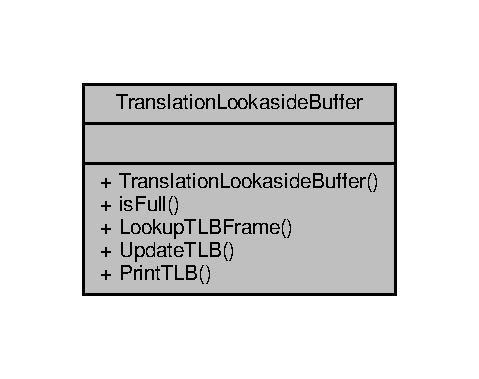
\includegraphics[width=230pt]{classTranslationLookasideBuffer__coll__graph}
\end{center}
\end{figure}
\subsection*{Public Member Functions}
\begin{DoxyCompactItemize}
\item 
\hyperlink{classTranslationLookasideBuffer_ad6df9fde44600dedcde0a0d7542e357a}{Translation\+Lookaside\+Buffer} ()
\begin{DoxyCompactList}\small\item\em Constructor for the T\+LB. \end{DoxyCompactList}\item 
bool \hyperlink{classTranslationLookasideBuffer_a6416b56aa9b1593b602281f3a81af091}{is\+Full} ()
\begin{DoxyCompactList}\small\item\em Determines whether the T\+LB is full. \end{DoxyCompactList}\item 
\hyperlink{structTLBReturnData__t}{T\+L\+B\+Return\+Data\+\_\+t} \hyperlink{classTranslationLookasideBuffer_a411659ccd7cb5b72a165bc69cc353e0a}{Lookup\+T\+L\+B\+Frame} (int pagenum)
\begin{DoxyCompactList}\small\item\em Searches the T\+LB for the frame. \end{DoxyCompactList}\item 
int \hyperlink{classTranslationLookasideBuffer_a68fe2b0deb2abb9854764471d7c2cba3}{Update\+T\+LB} (int pagenum, int framenum)
\begin{DoxyCompactList}\small\item\em Update the T\+LB with a new page/frame combination. \end{DoxyCompactList}\item 
void \hyperlink{classTranslationLookasideBuffer_a1f92817ce0487d710c6ef5b0176dd358}{Print\+T\+LB} ()
\begin{DoxyCompactList}\small\item\em Print the T\+LB. \end{DoxyCompactList}\end{DoxyCompactItemize}


\subsection{Detailed Description}


Definition at line \hyperlink{memory_8h_source_l00203}{203} of file \hyperlink{memory_8h_source}{memory.\+h}.



\subsection{Constructor \& Destructor Documentation}
\index{Translation\+Lookaside\+Buffer@{Translation\+Lookaside\+Buffer}!Translation\+Lookaside\+Buffer@{Translation\+Lookaside\+Buffer}}
\index{Translation\+Lookaside\+Buffer@{Translation\+Lookaside\+Buffer}!Translation\+Lookaside\+Buffer@{Translation\+Lookaside\+Buffer}}
\subsubsection[{\texorpdfstring{Translation\+Lookaside\+Buffer()}{TranslationLookasideBuffer()}}]{\setlength{\rightskip}{0pt plus 5cm}Translation\+Lookaside\+Buffer\+::\+Translation\+Lookaside\+Buffer (
\begin{DoxyParamCaption}
{}
\end{DoxyParamCaption}
)}\hypertarget{classTranslationLookasideBuffer_ad6df9fde44600dedcde0a0d7542e357a}{}\label{classTranslationLookasideBuffer_ad6df9fde44600dedcde0a0d7542e357a}


Constructor for the T\+LB. 



Definition at line \hyperlink{memory_8cpp_source_l00198}{198} of file \hyperlink{memory_8cpp_source}{memory.\+cpp}.



\subsection{Member Function Documentation}
\index{Translation\+Lookaside\+Buffer@{Translation\+Lookaside\+Buffer}!is\+Full@{is\+Full}}
\index{is\+Full@{is\+Full}!Translation\+Lookaside\+Buffer@{Translation\+Lookaside\+Buffer}}
\subsubsection[{\texorpdfstring{is\+Full()}{isFull()}}]{\setlength{\rightskip}{0pt plus 5cm}bool Translation\+Lookaside\+Buffer\+::is\+Full (
\begin{DoxyParamCaption}
{}
\end{DoxyParamCaption}
)}\hypertarget{classTranslationLookasideBuffer_a6416b56aa9b1593b602281f3a81af091}{}\label{classTranslationLookasideBuffer_a6416b56aa9b1593b602281f3a81af091}


Determines whether the T\+LB is full. 


\begin{DoxyRetVals}{Return values}
{\em bool} & True/false depending on status of T\+LB \\
\hline
\end{DoxyRetVals}


Definition at line \hyperlink{memory_8cpp_source_l00206}{206} of file \hyperlink{memory_8cpp_source}{memory.\+cpp}.

\index{Translation\+Lookaside\+Buffer@{Translation\+Lookaside\+Buffer}!Lookup\+T\+L\+B\+Frame@{Lookup\+T\+L\+B\+Frame}}
\index{Lookup\+T\+L\+B\+Frame@{Lookup\+T\+L\+B\+Frame}!Translation\+Lookaside\+Buffer@{Translation\+Lookaside\+Buffer}}
\subsubsection[{\texorpdfstring{Lookup\+T\+L\+B\+Frame(int pagenum)}{LookupTLBFrame(int pagenum)}}]{\setlength{\rightskip}{0pt plus 5cm}{\bf T\+L\+B\+Return\+Data\+\_\+t} Translation\+Lookaside\+Buffer\+::\+Lookup\+T\+L\+B\+Frame (
\begin{DoxyParamCaption}
\item[{int}]{pagenum}
\end{DoxyParamCaption}
)}\hypertarget{classTranslationLookasideBuffer_a411659ccd7cb5b72a165bc69cc353e0a}{}\label{classTranslationLookasideBuffer_a411659ccd7cb5b72a165bc69cc353e0a}


Searches the T\+LB for the frame. 


\begin{DoxyRetVals}{Return values}
{\em \hyperlink{structTLBReturnData__t}{T\+L\+B\+Return\+Data\+\_\+t}} & Returns frame number, or -\/1 if a T\+LB miss \\
\hline
\end{DoxyRetVals}


Definition at line \hyperlink{memory_8cpp_source_l00213}{213} of file \hyperlink{memory_8cpp_source}{memory.\+cpp}.

\index{Translation\+Lookaside\+Buffer@{Translation\+Lookaside\+Buffer}!Print\+T\+LB@{Print\+T\+LB}}
\index{Print\+T\+LB@{Print\+T\+LB}!Translation\+Lookaside\+Buffer@{Translation\+Lookaside\+Buffer}}
\subsubsection[{\texorpdfstring{Print\+T\+L\+B()}{PrintTLB()}}]{\setlength{\rightskip}{0pt plus 5cm}void Translation\+Lookaside\+Buffer\+::\+Print\+T\+LB (
\begin{DoxyParamCaption}
{}
\end{DoxyParamCaption}
)}\hypertarget{classTranslationLookasideBuffer_a1f92817ce0487d710c6ef5b0176dd358}{}\label{classTranslationLookasideBuffer_a1f92817ce0487d710c6ef5b0176dd358}


Print the T\+LB. 



Definition at line \hyperlink{memory_8cpp_source_l00261}{261} of file \hyperlink{memory_8cpp_source}{memory.\+cpp}.

\index{Translation\+Lookaside\+Buffer@{Translation\+Lookaside\+Buffer}!Update\+T\+LB@{Update\+T\+LB}}
\index{Update\+T\+LB@{Update\+T\+LB}!Translation\+Lookaside\+Buffer@{Translation\+Lookaside\+Buffer}}
\subsubsection[{\texorpdfstring{Update\+T\+L\+B(int pagenum, int framenum)}{UpdateTLB(int pagenum, int framenum)}}]{\setlength{\rightskip}{0pt plus 5cm}int Translation\+Lookaside\+Buffer\+::\+Update\+T\+LB (
\begin{DoxyParamCaption}
\item[{int}]{pagenum, }
\item[{int}]{framenum}
\end{DoxyParamCaption}
)}\hypertarget{classTranslationLookasideBuffer_a68fe2b0deb2abb9854764471d7c2cba3}{}\label{classTranslationLookasideBuffer_a68fe2b0deb2abb9854764471d7c2cba3}


Update the T\+LB with a new page/frame combination. 


\begin{DoxyParams}{Parameters}
{\em int} & Page number to cache \\
\hline
{\em int} & Frame number to cache \\
\hline
\end{DoxyParams}

\begin{DoxyRetVals}{Return values}
{\em int} & The index into which page/frame combo was hashed \\
\hline
\end{DoxyRetVals}


Definition at line \hyperlink{memory_8cpp_source_l00227}{227} of file \hyperlink{memory_8cpp_source}{memory.\+cpp}.



The documentation for this class was generated from the following files\+:\begin{DoxyCompactItemize}
\item 
src/\hyperlink{memory_8h}{memory.\+h}\item 
src/\hyperlink{memory_8cpp}{memory.\+cpp}\end{DoxyCompactItemize}

\chapter{File Documentation}
\hypertarget{main_8cpp}{}\section{src/main.cpp File Reference}
\label{main_8cpp}\index{src/main.\+cpp@{src/main.\+cpp}}
{\ttfamily \#include $<$iostream$>$}\\*
{\ttfamily \#include $<$fstream$>$}\\*
{\ttfamily \#include $<$sstream$>$}\\*
{\ttfamily \#include $<$cstdio$>$}\\*
{\ttfamily \#include \char`\"{}memory.\+h\char`\"{}}\\*
Include dependency graph for main.\+cpp\+:\nopagebreak
\begin{figure}[H]
\begin{center}
\leavevmode
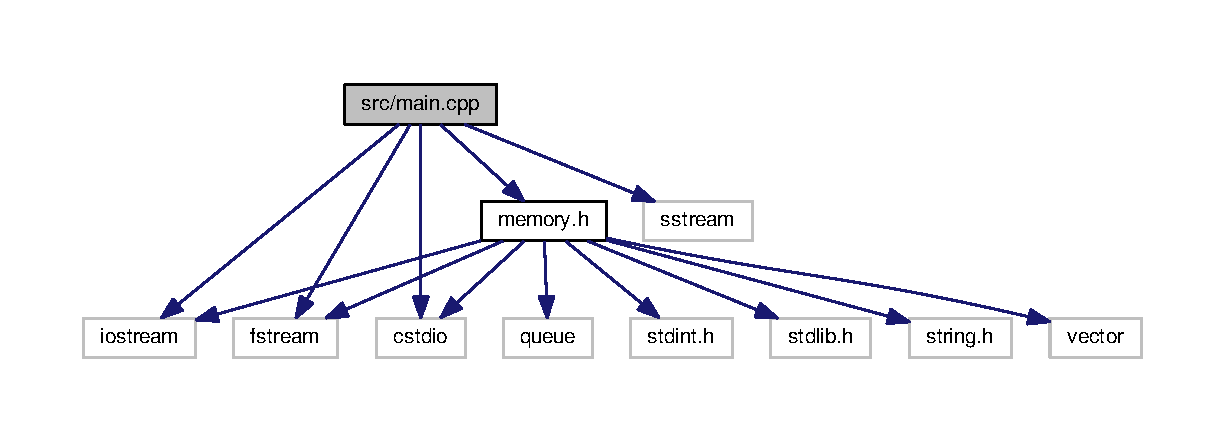
\includegraphics[width=350pt]{main_8cpp__incl}
\end{center}
\end{figure}
\subsection*{Macros}
\begin{DoxyCompactItemize}
\item 
\#define \hyperlink{main_8cpp_a3d58a37eb1401f1e1e0a2e43a28e0675}{I\+N\+P\+U\+T\+\_\+\+FN}~\char`\"{}addresses.\+txt\char`\"{}
\end{DoxyCompactItemize}
\subsection*{Functions}
\begin{DoxyCompactItemize}
\item 
void \hyperlink{main_8cpp_a5aa22abf10bfd6c47d6f04571ea77f1d}{Run\+Physical\+Memory\+Tests} ()
\item 
void \hyperlink{main_8cpp_a9d50d2049f7ee3c00984500c882ddde9}{Run\+Address\+Conversion\+Tests} ()
\item 
void \hyperlink{main_8cpp_a31aaac7e09dbfca2c888cb8e319fcdbd}{Run\+Paging\+Tests} ()
\item 
void \hyperlink{main_8cpp_ac5347a09d49e669bd79b50bf65d74e7d}{Run\+Full\+Memory\+Tests} ()
\item 
void \hyperlink{main_8cpp_a42ef34a387e48b6661322f8f1d6da730}{Execute\+From\+File} ()
\item 
int \hyperlink{main_8cpp_ae66f6b31b5ad750f1fe042a706a4e3d4}{main} ()
\end{DoxyCompactItemize}


\subsection{Macro Definition Documentation}
\index{main.\+cpp@{main.\+cpp}!I\+N\+P\+U\+T\+\_\+\+FN@{I\+N\+P\+U\+T\+\_\+\+FN}}
\index{I\+N\+P\+U\+T\+\_\+\+FN@{I\+N\+P\+U\+T\+\_\+\+FN}!main.\+cpp@{main.\+cpp}}
\subsubsection[{\texorpdfstring{I\+N\+P\+U\+T\+\_\+\+FN}{INPUT_FN}}]{\setlength{\rightskip}{0pt plus 5cm}\#define I\+N\+P\+U\+T\+\_\+\+FN~\char`\"{}addresses.\+txt\char`\"{}}\hypertarget{main_8cpp_a3d58a37eb1401f1e1e0a2e43a28e0675}{}\label{main_8cpp_a3d58a37eb1401f1e1e0a2e43a28e0675}


Definition at line \hyperlink{main_8cpp_source_l00008}{8} of file \hyperlink{main_8cpp_source}{main.\+cpp}.



\subsection{Function Documentation}
\index{main.\+cpp@{main.\+cpp}!Execute\+From\+File@{Execute\+From\+File}}
\index{Execute\+From\+File@{Execute\+From\+File}!main.\+cpp@{main.\+cpp}}
\subsubsection[{\texorpdfstring{Execute\+From\+File()}{ExecuteFromFile()}}]{\setlength{\rightskip}{0pt plus 5cm}void Execute\+From\+File (
\begin{DoxyParamCaption}
{}
\end{DoxyParamCaption}
)}\hypertarget{main_8cpp_a42ef34a387e48b6661322f8f1d6da730}{}\label{main_8cpp_a42ef34a387e48b6661322f8f1d6da730}


Definition at line \hyperlink{main_8cpp_source_l00022}{22} of file \hyperlink{main_8cpp_source}{main.\+cpp}.

\index{main.\+cpp@{main.\+cpp}!main@{main}}
\index{main@{main}!main.\+cpp@{main.\+cpp}}
\subsubsection[{\texorpdfstring{main()}{main()}}]{\setlength{\rightskip}{0pt plus 5cm}int main (
\begin{DoxyParamCaption}
{}
\end{DoxyParamCaption}
)}\hypertarget{main_8cpp_ae66f6b31b5ad750f1fe042a706a4e3d4}{}\label{main_8cpp_ae66f6b31b5ad750f1fe042a706a4e3d4}


Definition at line \hyperlink{main_8cpp_source_l00017}{17} of file \hyperlink{main_8cpp_source}{main.\+cpp}.

\index{main.\+cpp@{main.\+cpp}!Run\+Address\+Conversion\+Tests@{Run\+Address\+Conversion\+Tests}}
\index{Run\+Address\+Conversion\+Tests@{Run\+Address\+Conversion\+Tests}!main.\+cpp@{main.\+cpp}}
\subsubsection[{\texorpdfstring{Run\+Address\+Conversion\+Tests()}{RunAddressConversionTests()}}]{\setlength{\rightskip}{0pt plus 5cm}void Run\+Address\+Conversion\+Tests (
\begin{DoxyParamCaption}
{}
\end{DoxyParamCaption}
)}\hypertarget{main_8cpp_a9d50d2049f7ee3c00984500c882ddde9}{}\label{main_8cpp_a9d50d2049f7ee3c00984500c882ddde9}


Definition at line \hyperlink{main_8cpp_source_l00092}{92} of file \hyperlink{main_8cpp_source}{main.\+cpp}.

\index{main.\+cpp@{main.\+cpp}!Run\+Full\+Memory\+Tests@{Run\+Full\+Memory\+Tests}}
\index{Run\+Full\+Memory\+Tests@{Run\+Full\+Memory\+Tests}!main.\+cpp@{main.\+cpp}}
\subsubsection[{\texorpdfstring{Run\+Full\+Memory\+Tests()}{RunFullMemoryTests()}}]{\setlength{\rightskip}{0pt plus 5cm}void Run\+Full\+Memory\+Tests (
\begin{DoxyParamCaption}
{}
\end{DoxyParamCaption}
)}\hypertarget{main_8cpp_ac5347a09d49e669bd79b50bf65d74e7d}{}\label{main_8cpp_ac5347a09d49e669bd79b50bf65d74e7d}


Definition at line \hyperlink{main_8cpp_source_l00050}{50} of file \hyperlink{main_8cpp_source}{main.\+cpp}.

\index{main.\+cpp@{main.\+cpp}!Run\+Paging\+Tests@{Run\+Paging\+Tests}}
\index{Run\+Paging\+Tests@{Run\+Paging\+Tests}!main.\+cpp@{main.\+cpp}}
\subsubsection[{\texorpdfstring{Run\+Paging\+Tests()}{RunPagingTests()}}]{\setlength{\rightskip}{0pt plus 5cm}void Run\+Paging\+Tests (
\begin{DoxyParamCaption}
{}
\end{DoxyParamCaption}
)}\hypertarget{main_8cpp_a31aaac7e09dbfca2c888cb8e319fcdbd}{}\label{main_8cpp_a31aaac7e09dbfca2c888cb8e319fcdbd}


Definition at line \hyperlink{main_8cpp_source_l00068}{68} of file \hyperlink{main_8cpp_source}{main.\+cpp}.

\index{main.\+cpp@{main.\+cpp}!Run\+Physical\+Memory\+Tests@{Run\+Physical\+Memory\+Tests}}
\index{Run\+Physical\+Memory\+Tests@{Run\+Physical\+Memory\+Tests}!main.\+cpp@{main.\+cpp}}
\subsubsection[{\texorpdfstring{Run\+Physical\+Memory\+Tests()}{RunPhysicalMemoryTests()}}]{\setlength{\rightskip}{0pt plus 5cm}void Run\+Physical\+Memory\+Tests (
\begin{DoxyParamCaption}
{}
\end{DoxyParamCaption}
)}\hypertarget{main_8cpp_a5aa22abf10bfd6c47d6f04571ea77f1d}{}\label{main_8cpp_a5aa22abf10bfd6c47d6f04571ea77f1d}


Definition at line \hyperlink{main_8cpp_source_l00102}{102} of file \hyperlink{main_8cpp_source}{main.\+cpp}.


\hypertarget{main_8cpp_source}{}\section{main.\+cpp}
\label{main_8cpp_source}\index{src/main.\+cpp@{src/main.\+cpp}}

\begin{DoxyCode}
00001 \textcolor{preprocessor}{#include <iostream>}
00002 \textcolor{preprocessor}{#include <fstream>}
00003 \textcolor{preprocessor}{#include <sstream>}
00004 \textcolor{preprocessor}{#include <cstdio>}
00005 \textcolor{preprocessor}{#include "\hyperlink{memory_8h}{memory.h}"}
00006 \textcolor{keyword}{using namespace }\hyperlink{namespacestd}{std};
00007 
\hypertarget{main_8cpp_source.tex_l00008}{}\hyperlink{main_8cpp_a3d58a37eb1401f1e1e0a2e43a28e0675}{00008} \textcolor{preprocessor}{#define INPUT\_FN "addresses.txt"}
00009 
00010 \textcolor{keywordtype}{void} \hyperlink{main_8cpp_a5aa22abf10bfd6c47d6f04571ea77f1d}{RunPhysicalMemoryTests}();
00011 \textcolor{keywordtype}{void} \hyperlink{main_8cpp_a9d50d2049f7ee3c00984500c882ddde9}{RunAddressConversionTests}();
00012 \textcolor{keywordtype}{void} \hyperlink{main_8cpp_a31aaac7e09dbfca2c888cb8e319fcdbd}{RunPagingTests}();
00013 \textcolor{keywordtype}{void} \hyperlink{main_8cpp_ac5347a09d49e669bd79b50bf65d74e7d}{RunFullMemoryTests}();
00014 
00015 \textcolor{keywordtype}{void} \hyperlink{main_8cpp_a42ef34a387e48b6661322f8f1d6da730}{ExecuteFromFile}();
00016 
\hypertarget{main_8cpp_source.tex_l00017}{}\hyperlink{main_8cpp_ae66f6b31b5ad750f1fe042a706a4e3d4}{00017} \textcolor{keywordtype}{int} \hyperlink{main_8cpp_ae66f6b31b5ad750f1fe042a706a4e3d4}{main}() \{
00018     \hyperlink{main_8cpp_a42ef34a387e48b6661322f8f1d6da730}{ExecuteFromFile}();
00019     \textcolor{keywordflow}{return} 0;
00020 \}
00021 
\hypertarget{main_8cpp_source.tex_l00022}{}\hyperlink{main_8cpp_a42ef34a387e48b6661322f8f1d6da730}{00022} \textcolor{keywordtype}{void} \hyperlink{main_8cpp_a42ef34a387e48b6661322f8f1d6da730}{ExecuteFromFile}() \{
00023     \hyperlink{classMemoryManager}{MemoryManager} mmu;
00024 
00025     std::ifstream infile(\hyperlink{main_8cpp_a3d58a37eb1401f1e1e0a2e43a28e0675}{INPUT\_FN});
00026     std::string line;
00027     \textcolor{keywordflow}{while}(std::getline(infile, line)) \{
00028         std::istringstream iss(line);
00029         \textcolor{keywordtype}{int} addr;
00030         
00031         \textcolor{keywordflow}{if}(!(iss >> addr))\{
00032             cout << \textcolor{stringliteral}{"I/O ERROR: Couldn't parse "} << iss << endl;
00033             exit(EXIT\_FAILURE);
00034         \}
00035         cout << \textcolor{stringliteral}{"Dereferencing address \{"} << addr << \textcolor{stringliteral}{"\}..."} << endl;
00036         \textcolor{keywordtype}{int} contents = mmu.\hyperlink{classMemoryManager_a4a716fc46ee321ebb25bd54bcc9d0524}{ReadMemory}(addr);
00037         cout << \textcolor{stringliteral}{"... found data ["} << contents << \textcolor{stringliteral}{"]"} << endl << endl;
00038     \}
00039 
00040     cout << endl << \textcolor{stringliteral}{"Contents of TLB:"} << endl;
00041     mmu.\hyperlink{classMemoryManager_a4bc5f491976e5253bf00a07a71b55ef6}{PrintTLB}();
00042     cout << endl << \textcolor{stringliteral}{"Contents of Page Table:"} << endl;
00043     mmu.\hyperlink{classMemoryManager_aa7437efdc1ebd09895d451e2c521857a}{PrintPageTable}();
00044     cout << endl << \textcolor{stringliteral}{"Contents of Page Table (Inverse):"} << endl;
00045     mmu.\hyperlink{classMemoryManager_a231141529c907c50de129169f16bedf1}{PrintInversePageTable}();
00046     cout << endl << \textcolor{stringliteral}{"Memory Access Statistics: "} << endl << endl;
00047     mmu.\hyperlink{classMemoryManager_ad0c7c13901cb9c6844aebf6bf9238c47}{PrintStats}();
00048 \}
00049 
\hypertarget{main_8cpp_source.tex_l00050}{}\hyperlink{main_8cpp_ac5347a09d49e669bd79b50bf65d74e7d}{00050} \textcolor{keywordtype}{void} \hyperlink{main_8cpp_ac5347a09d49e669bd79b50bf65d74e7d}{RunFullMemoryTests}() \{
00051     \hyperlink{classMemoryManager}{MemoryManager} mmu;
00052     \textcolor{comment}{// Fill the memory with the first 8 frames}
00053     
00054     \textcolor{keywordflow}{for}(\textcolor{keywordtype}{int} i = 1; i < 4095-255; i = i + 256) \{
00055         mmu.\hyperlink{classMemoryManager_a4a716fc46ee321ebb25bd54bcc9d0524}{ReadMemory}(i);
00056         mmu.\hyperlink{classMemoryManager_ae7bbb5231788516ca34caca3d428b0ef}{PrintAll}();
00057     \}
00058     mmu.\hyperlink{classMemoryManager_a4a716fc46ee321ebb25bd54bcc9d0524}{ReadMemory}(3555);
00059     mmu.\hyperlink{classMemoryManager_ae7bbb5231788516ca34caca3d428b0ef}{PrintAll}();
00060     mmu.\hyperlink{classMemoryManager_a4a716fc46ee321ebb25bd54bcc9d0524}{ReadMemory}(5);
00061     mmu.\hyperlink{classMemoryManager_ae7bbb5231788516ca34caca3d428b0ef}{PrintAll}();
00062     mmu.\hyperlink{classMemoryManager_a4a716fc46ee321ebb25bd54bcc9d0524}{ReadMemory}(2050);
00063     mmu.\hyperlink{classMemoryManager_ae7bbb5231788516ca34caca3d428b0ef}{PrintAll}();
00064     mmu.\hyperlink{classMemoryManager_a4a716fc46ee321ebb25bd54bcc9d0524}{ReadMemory}(2050);
00065     mmu.\hyperlink{classMemoryManager_ae7bbb5231788516ca34caca3d428b0ef}{PrintAll}();
00066 \}
00067 
\hypertarget{main_8cpp_source.tex_l00068}{}\hyperlink{main_8cpp_a31aaac7e09dbfca2c888cb8e319fcdbd}{00068} \textcolor{keywordtype}{void} \hyperlink{main_8cpp_a31aaac7e09dbfca2c888cb8e319fcdbd}{RunPagingTests}() \{
00069     \hyperlink{classMemoryManager}{MemoryManager} mmu;
00070     \textcolor{keywordtype}{char} result;
00071     \textcolor{keywordtype}{int} addr;
00072 
00073     addr = 1;
00074     result = mmu.\hyperlink{classMemoryManager_a4a716fc46ee321ebb25bd54bcc9d0524}{ReadMemory}(addr);
00075     printf(\textcolor{stringliteral}{"Retrieved \{%d\} from virtual address \{%d\}\(\backslash\)n\(\backslash\)n"}, result, addr);
00076     \textcolor{comment}{// The page table should have frame 0 assigned to page 0}
00077     \textcolor{comment}{// mmu.PrintPageTable();}
00078 
00079     addr = 513;
00080     result = mmu.\hyperlink{classMemoryManager_a4a716fc46ee321ebb25bd54bcc9d0524}{ReadMemory}(addr);
00081     printf(\textcolor{stringliteral}{"Retrieved \{%d\} from virtual address \{%d\}\(\backslash\)n\(\backslash\)n"}, result, addr);
00082     \textcolor{comment}{// mmu.PrintPageTable();}
00083 
00084     addr = 515;
00085     result = mmu.\hyperlink{classMemoryManager_a4a716fc46ee321ebb25bd54bcc9d0524}{ReadMemory}(addr);
00086     printf(\textcolor{stringliteral}{"Retrieved \{%d\} from virtual address \{%d\}\(\backslash\)n\(\backslash\)n"}, result, addr);
00087     \textcolor{comment}{// result = mmu.ReadMemory(515);}
00088     mmu.\hyperlink{classMemoryManager_aa7437efdc1ebd09895d451e2c521857a}{PrintPageTable}();
00089 
00090 \}
00091 
\hypertarget{main_8cpp_source.tex_l00092}{}\hyperlink{main_8cpp_a9d50d2049f7ee3c00984500c882ddde9}{00092} \textcolor{keywordtype}{void} \hyperlink{main_8cpp_a9d50d2049f7ee3c00984500c882ddde9}{RunAddressConversionTests}()\{ 
00093     \hyperlink{structMemoryPairAddress__t}{MemoryPairAddress\_t} m1 = \hyperlink{memory_8cpp_a90bdb77a86b4a78c22b50e250b77d9ad}{ConvertAddressFormat}(2096);
00094     \hyperlink{memory_8cpp_ac93b824d9e950d90189b96ba89151512}{PrintMemoryPairAddress}(m1);
00095 
00096     m1 = \hyperlink{memory_8cpp_a90bdb77a86b4a78c22b50e250b77d9ad}{ConvertAddressFormat}(4095);
00097     \hyperlink{memory_8cpp_ac93b824d9e950d90189b96ba89151512}{PrintMemoryPairAddress}(m1);
00098 
00099     m1 = \hyperlink{memory_8cpp_a90bdb77a86b4a78c22b50e250b77d9ad}{ConvertAddressFormat}(6);
00100     \hyperlink{memory_8cpp_ac93b824d9e950d90189b96ba89151512}{PrintMemoryPairAddress}(m1);
00101 \}
\hypertarget{main_8cpp_source.tex_l00102}{}\hyperlink{main_8cpp_a5aa22abf10bfd6c47d6f04571ea77f1d}{00102} \textcolor{keywordtype}{void} \hyperlink{main_8cpp_a5aa22abf10bfd6c47d6f04571ea77f1d}{RunPhysicalMemoryTests}()\{
00103     \hyperlink{classPhysicalMemory}{PhysicalMemory} pmem;
00104     pmem.\hyperlink{classPhysicalMemory_a2d6b5c45f2377838a76e58b2c083610a}{GetMemoryContents}(0, 100);
00105     pmem.\hyperlink{classPhysicalMemory_a2d6b5c45f2377838a76e58b2c083610a}{GetMemoryContents}(1, 100);
00106     pmem.\hyperlink{classPhysicalMemory_a2d6b5c45f2377838a76e58b2c083610a}{GetMemoryContents}(2, 100);
00107     pmem.\hyperlink{classPhysicalMemory_a2d6b5c45f2377838a76e58b2c083610a}{GetMemoryContents}(3, 100);
00108 
00109     pmem.\hyperlink{classPhysicalMemory_a2d6b5c45f2377838a76e58b2c083610a}{GetMemoryContents}(5, 100);
00110     pmem.\hyperlink{classPhysicalMemory_a2d6b5c45f2377838a76e58b2c083610a}{GetMemoryContents}(6, 100);
00111     pmem.\hyperlink{classPhysicalMemory_a2d6b5c45f2377838a76e58b2c083610a}{GetMemoryContents}(7, 100);
00112     pmem.\hyperlink{classPhysicalMemory_a2d6b5c45f2377838a76e58b2c083610a}{GetMemoryContents}(1, 100);
00113     pmem.\hyperlink{classPhysicalMemory_a2d6b5c45f2377838a76e58b2c083610a}{GetMemoryContents}(2, 100);
00114     pmem.\hyperlink{classPhysicalMemory_a2d6b5c45f2377838a76e58b2c083610a}{GetMemoryContents}(3, 100);
00115     pmem.\hyperlink{classPhysicalMemory_a2d6b5c45f2377838a76e58b2c083610a}{GetMemoryContents}(4, 100);
00116 
00117     pmem.\hyperlink{classPhysicalMemory_a2d6b5c45f2377838a76e58b2c083610a}{GetMemoryContents}(5, 100);
00118     pmem.\hyperlink{classPhysicalMemory_a2d6b5c45f2377838a76e58b2c083610a}{GetMemoryContents}(6, 100);
00119 
00120     \textcolor{comment}{// pmem.GetMemoryContents(0, 300);}
00121 
00122     \textcolor{comment}{// printf("Least used: %d\(\backslash\)n", pmem.FindLRUFrame());}
00123     printf(\textcolor{stringliteral}{"Full?: %d\(\backslash\)n"}, pmem.\hyperlink{classPhysicalMemory_acde26e332e20349baa6c409b88635258}{isFull}());
00124     printf(\textcolor{stringliteral}{"First available frame: %d\(\backslash\)n"}, pmem.\hyperlink{classPhysicalMemory_a41ba2824ae9550b68036536d94ae8b32}{FindFirstFrame}());
00125 
00126 \}
\end{DoxyCode}

\hypertarget{memory_8cpp}{}\section{src/memory.cpp File Reference}
\label{memory_8cpp}\index{src/memory.\+cpp@{src/memory.\+cpp}}
{\ttfamily \#include \char`\"{}memory.\+h\char`\"{}}\\*
Include dependency graph for memory.\+cpp\+:\nopagebreak
\begin{figure}[H]
\begin{center}
\leavevmode
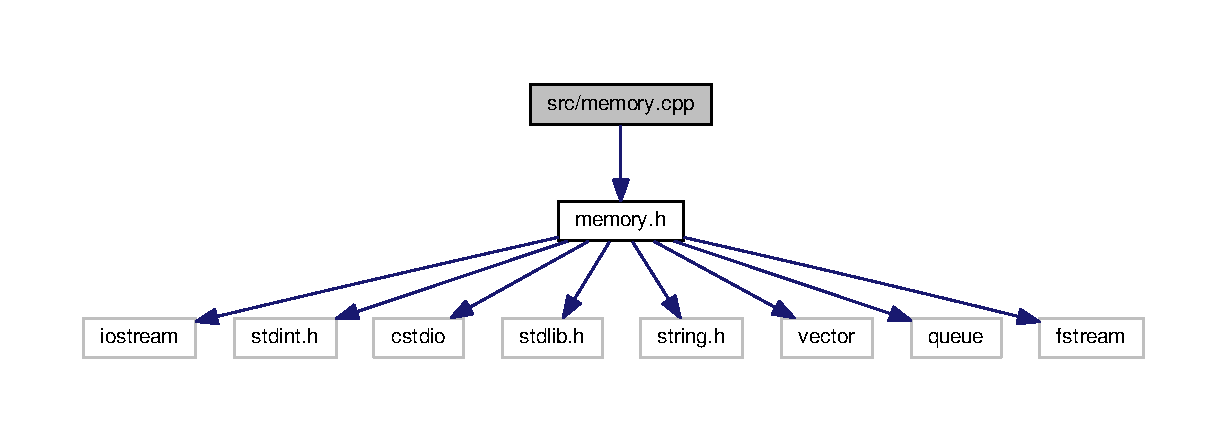
\includegraphics[width=350pt]{memory_8cpp__incl}
\end{center}
\end{figure}
\subsection*{Functions}
\begin{DoxyCompactItemize}
\item 
\hyperlink{structMemoryPairAddress__t}{Memory\+Pair\+Address\+\_\+t} \hyperlink{memory_8cpp_a90bdb77a86b4a78c22b50e250b77d9ad}{Convert\+Address\+Format} (int addr)
\begin{DoxyCompactList}\small\item\em Convert a base-\/10 address to (P, d) format. \end{DoxyCompactList}\item 
void \hyperlink{memory_8cpp_ac93b824d9e950d90189b96ba89151512}{Print\+Memory\+Pair\+Address} (\hyperlink{structMemoryPairAddress__t}{Memory\+Pair\+Address\+\_\+t} mempair)
\end{DoxyCompactItemize}


\subsection{Function Documentation}
\index{memory.\+cpp@{memory.\+cpp}!Convert\+Address\+Format@{Convert\+Address\+Format}}
\index{Convert\+Address\+Format@{Convert\+Address\+Format}!memory.\+cpp@{memory.\+cpp}}
\subsubsection[{\texorpdfstring{Convert\+Address\+Format(int addr)}{ConvertAddressFormat(int addr)}}]{\setlength{\rightskip}{0pt plus 5cm}{\bf Memory\+Pair\+Address\+\_\+t} Convert\+Address\+Format (
\begin{DoxyParamCaption}
\item[{int}]{addr}
\end{DoxyParamCaption}
)}\hypertarget{memory_8cpp_a90bdb77a86b4a78c22b50e250b77d9ad}{}\label{memory_8cpp_a90bdb77a86b4a78c22b50e250b77d9ad}


Convert a base-\/10 address to (P, d) format. 


\begin{DoxyParams}{Parameters}
{\em int} & base-\/10 address to translate \\
\hline
\end{DoxyParams}

\begin{DoxyRetVals}{Return values}
{\em \hyperlink{structMemoryPairAddress__t}{Memory\+Pair\+Address\+\_\+t}} & (P, d) pair corresponding to the address \\
\hline
\end{DoxyRetVals}


Definition at line \hyperlink{memory_8cpp_source_l00457}{457} of file \hyperlink{memory_8cpp_source}{memory.\+cpp}.

\index{memory.\+cpp@{memory.\+cpp}!Print\+Memory\+Pair\+Address@{Print\+Memory\+Pair\+Address}}
\index{Print\+Memory\+Pair\+Address@{Print\+Memory\+Pair\+Address}!memory.\+cpp@{memory.\+cpp}}
\subsubsection[{\texorpdfstring{Print\+Memory\+Pair\+Address(\+Memory\+Pair\+Address\+\_\+t mempair)}{PrintMemoryPairAddress(MemoryPairAddress_t mempair)}}]{\setlength{\rightskip}{0pt plus 5cm}void Print\+Memory\+Pair\+Address (
\begin{DoxyParamCaption}
\item[{{\bf Memory\+Pair\+Address\+\_\+t}}]{mempair}
\end{DoxyParamCaption}
)}\hypertarget{memory_8cpp_ac93b824d9e950d90189b96ba89151512}{}\label{memory_8cpp_ac93b824d9e950d90189b96ba89151512}


Definition at line \hyperlink{memory_8cpp_source_l00465}{465} of file \hyperlink{memory_8cpp_source}{memory.\+cpp}.


\hypertarget{memory_8cpp_source}{}\section{memory.\+cpp}
\label{memory_8cpp_source}\index{src/memory.\+cpp@{src/memory.\+cpp}}

\begin{DoxyCode}
00001 \textcolor{preprocessor}{#include "\hyperlink{memory_8h}{memory.h}"}
00002 \textcolor{keyword}{using namespace }\hyperlink{namespacestd}{std};
00003 \textcolor{comment}{/*=======================================}
00004 \textcolor{comment}{=            Physical Memory            =}
00005 \textcolor{comment}{=======================================*/}
00006 
\hypertarget{memory_8cpp_source.tex_l00007}{}\hyperlink{classPhysicalMemory_ad7fefaba61061c7339164836c6c02eaa}{00007} \hyperlink{classPhysicalMemory_ad7fefaba61061c7339164836c6c02eaa}{PhysicalMemory::PhysicalMemory}() \{
00008     \textcolor{keywordflow}{for}(\textcolor{keywordtype}{int} i = 0; i < n\_frames; i++) \{
00009         \textcolor{keywordflow}{for}(\textcolor{keywordtype}{int} j = 0; j < frame\_size; j++) \{
00010             memory[i][j] = 0x00;
00011         \}
00012         occupied[i] = 0x00;
00013     \}
00014 \}
00015 
00016 \textcolor{comment}{// Determine if the memory is full}
\hypertarget{memory_8cpp_source.tex_l00017}{}\hyperlink{classPhysicalMemory_acde26e332e20349baa6c409b88635258}{00017} \textcolor{keywordtype}{bool} \hyperlink{classPhysicalMemory_acde26e332e20349baa6c409b88635258}{PhysicalMemory::isFull}() \{
00018     
00019     \textcolor{keywordflow}{for}(\textcolor{keywordtype}{int} i = 0; i < n\_frames; i++) \{
00020         \textcolor{keywordflow}{if}(occupied[i] == 0) \textcolor{keywordflow}{return} \textcolor{keyword}{false};
00021     \}
00022     \textcolor{keywordflow}{return} \textcolor{keyword}{true};
00023 
00024 \}
00025 
00026 \textcolor{comment}{// Find the first available frame}
\hypertarget{memory_8cpp_source.tex_l00027}{}\hyperlink{classPhysicalMemory_a41ba2824ae9550b68036536d94ae8b32}{00027} \textcolor{keywordtype}{int} \hyperlink{classPhysicalMemory_a41ba2824ae9550b68036536d94ae8b32}{PhysicalMemory::FindFirstFrame}() \{
00028     \textcolor{keywordflow}{for}(\textcolor{keywordtype}{int} i = 0; i < n\_frames; i++) \{
00029         \textcolor{keywordflow}{if}(occupied[i] == 0) \{
00030             \textcolor{keywordflow}{return} i;
00031         \}
00032     \}
00033     \textcolor{keywordflow}{return} -1;
00034 \}
00035 
00036 \textcolor{comment}{// Return the contents of memory at a give frame and offset}
\hypertarget{memory_8cpp_source.tex_l00037}{}\hyperlink{classPhysicalMemory_a2d6b5c45f2377838a76e58b2c083610a}{00037} \textcolor{keywordtype}{char} \hyperlink{classPhysicalMemory_a2d6b5c45f2377838a76e58b2c083610a}{PhysicalMemory::GetMemoryContents}(\textcolor{keywordtype}{int} frame, \textcolor{keywordtype}{int} offset) \{
00038     \textcolor{keywordflow}{if}(frame >= n\_frames) \{
00039         fprintf(stderr, \textcolor{stringliteral}{"%s %d\(\backslash\)n"}, \textcolor{stringliteral}{"MEM\_ERROR1: invalid frame #: "},frame);
00040         exit(EXIT\_FAILURE);
00041     \}
00042     \textcolor{keywordflow}{if}(offset >= frame\_size) \{
00043         fprintf(stderr, \textcolor{stringliteral}{"%s %d\(\backslash\)n"}, \textcolor{stringliteral}{"MEM\_ERROR2: invalid offset #: "},offset);
00044         exit(EXIT\_FAILURE);
00045     \}
00046 
00047     \textcolor{keywordflow}{return} memory[frame][offset];
00048 \}
00049 
\hypertarget{memory_8cpp_source.tex_l00050}{}\hyperlink{classPhysicalMemory_a70cb4ae5b23f04cb347ac93cc9fc1028}{00050} \textcolor{keywordtype}{void} \hyperlink{classPhysicalMemory_a70cb4ae5b23f04cb347ac93cc9fc1028}{PhysicalMemory::PageIn}(\textcolor{keywordtype}{int} frame, \textcolor{keywordtype}{char} pagein[
      \hyperlink{memory_8h_af9b1b2ba12857a4bf11289dac8c5462d}{FRAME\_SIZE}]) \{
00051     \textcolor{keywordflow}{if}(frame >= \hyperlink{memory_8h_a0b0ce802de0cae773522024d7626b007}{N\_FRAMES}) \{
00052         fprintf(stderr, \textcolor{stringliteral}{"%s %d\(\backslash\)n"}, \textcolor{stringliteral}{"MEM\_ERROR3: invalid frame #: "}, frame);
00053         exit(EXIT\_FAILURE);
00054     \}
00055     \textcolor{keywordflow}{for}(\textcolor{keywordtype}{int} i = 0; i < \hyperlink{memory_8h_af9b1b2ba12857a4bf11289dac8c5462d}{FRAME\_SIZE}; i++) \{
00056         memory[frame][i] = pagein[i];
00057     \}
00058     occupied[frame] = 1;
00059 \}
00060 
\hypertarget{memory_8cpp_source.tex_l00061}{}\hyperlink{classPhysicalMemory_a6e1cf83f35ab25e879630783ebaecff3}{00061} \textcolor{keywordtype}{void} \hyperlink{classPhysicalMemory_a6e1cf83f35ab25e879630783ebaecff3}{PhysicalMemory::PageOut}(\textcolor{keywordtype}{int} frame) \{
00062     \textcolor{keywordflow}{if}(frame < 0 || frame >= \hyperlink{memory_8h_a0b0ce802de0cae773522024d7626b007}{N\_FRAMES}) \{
00063         fprintf(stderr, \textcolor{stringliteral}{"MEM\_ERROR4: invalid frame # %d\(\backslash\)n"},frame);
00064         exit(EXIT\_FAILURE);
00065     \}
00066     \textcolor{keywordflow}{for}(\textcolor{keywordtype}{int} i = 0; i < \hyperlink{memory_8h_af9b1b2ba12857a4bf11289dac8c5462d}{FRAME\_SIZE}; i++) \{
00067         memory[frame][i] = 0x00;
00068     \}
00069     occupied[frame] = 0;
00070 \}
00071 \textcolor{comment}{/*=====  End of Physical Memory  ======*/}
00072 
00073 
00074 
00075 
00076 
00077 
00078 
00079 
00080 \textcolor{comment}{/*==================================}
00081 \textcolor{comment}{=            Page Table            =}
00082 \textcolor{comment}{==================================*/}
00083 
00084 \textcolor{comment}{// Page Table Constructor}
\hypertarget{memory_8cpp_source.tex_l00085}{}\hyperlink{classPageTable_a75c92e794fd3f5397d2499d54dac22c9}{00085} \hyperlink{classPageTable_a75c92e794fd3f5397d2499d54dac22c9}{PageTable::PageTable}() \{
00086     \textcolor{keywordflow}{for}(\textcolor{keywordtype}{int} i = 0; i < pgtable\_entries; i++) \{
00087         pgtable[i] = -1;
00088         valid[i] = 0;
00089     \}
00090 \}
00091 
00092 \textcolor{comment}{// Lookup a page number and return the corresponding frame}
\hypertarget{memory_8cpp_source.tex_l00093}{}\hyperlink{classPageTable_a2590af90445c76b97420da95cf7210ec}{00093} \textcolor{keywordtype}{int} \hyperlink{classPageTable_a2590af90445c76b97420da95cf7210ec}{PageTable::LookupPage}(\textcolor{keywordtype}{int} pagenum) \{
00094     \textcolor{keywordflow}{if}(pagenum >= pgtable\_entries) \{
00095         fprintf(stderr, \textcolor{stringliteral}{"%s %d\(\backslash\)n"}, \textcolor{stringliteral}{"PT\_ERROR: invalid page #: "}, pagenum );
00096         exit(EXIT\_FAILURE);
00097     \}
00098     UpdateLRUList(pagenum);
00099     \textcolor{keywordflow}{return} pgtable[pagenum];
00100 \}
\hypertarget{memory_8cpp_source.tex_l00101}{}\hyperlink{classPageTable_a3444b04644cb833bfd2a9b615704e6a1}{00101} \textcolor{keywordtype}{int} \hyperlink{classPageTable_a3444b04644cb833bfd2a9b615704e6a1}{PageTable::LookupPage\_no\_LRU}(\textcolor{keywordtype}{int} pagenum)\{
00102     \textcolor{keywordflow}{if}(pagenum >= pgtable\_entries) \{
00103         fprintf(stderr, \textcolor{stringliteral}{"%s %d\(\backslash\)n"}, \textcolor{stringliteral}{"PT\_ERROR: invalid page #: "}, pagenum );
00104         exit(EXIT\_FAILURE);
00105     \}
00106     \textcolor{keywordflow}{return} pgtable[pagenum];
00107 \}
00108 \textcolor{comment}{// Set a value of the page table}
\hypertarget{memory_8cpp_source.tex_l00109}{}\hyperlink{classPageTable_ac961a37f5dde09c3addce2fcd118f24d}{00109} \textcolor{keywordtype}{void} \hyperlink{classPageTable_ac961a37f5dde09c3addce2fcd118f24d}{PageTable::SetPageToFrame}(\textcolor{keywordtype}{int} pagenum, \textcolor{keywordtype}{int} framenum) \{
00110     \textcolor{keywordflow}{if}(pagenum >= pgtable\_entries || framenum >= \hyperlink{memory_8h_af9b1b2ba12857a4bf11289dac8c5462d}{FRAME\_SIZE}) \{
00111         fprintf(stderr, \textcolor{stringliteral}{"PT\_ERROR: Invalid Page/Frame Combination: Page: %d , Frame: %d\(\backslash\)n"}, pagenum, 
      framenum);
00112         exit(EXIT\_FAILURE);
00113     \}
00114     pgtable[pagenum] = framenum;
00115     valid[pagenum] = 1;
00116 \}
00117 
\hypertarget{memory_8cpp_source.tex_l00118}{}\hyperlink{classPageTable_ae8c5d4a967b4d8d45e8d4e517f618f70}{00118} \textcolor{keywordtype}{void} \hyperlink{classPageTable_ae8c5d4a967b4d8d45e8d4e517f618f70}{PageTable::PageOut\_table}(\textcolor{keywordtype}{int} pagenum) \{
00119     \textcolor{keywordflow}{if}(pagenum >= pgtable\_entries) \{
00120         fprintf(stderr, \textcolor{stringliteral}{"PT\_ERROR: Invalid Page #: %d"}, pagenum);
00121         exit(EXIT\_FAILURE);
00122     \}
00123     pgtable[pagenum] = -1;
00124     valid[pagenum] = 0;
00125 
00126     \textcolor{keywordtype}{int} lrusize = LRU\_list.size();
00127     \textcolor{keywordflow}{for}(\textcolor{keywordtype}{int} i = 0; i < lrusize; i++) \{
00128         \textcolor{keywordflow}{if} (LRU\_list[i] == pagenum) \{
00129             LRU\_list.erase(LRU\_list.begin() + i);
00130             \textcolor{keywordflow}{break};
00131         \}
00132     \} 
00133 \}
00134 
\hypertarget{memory_8cpp_source.tex_l00135}{}\hyperlink{classPageTable_ac43e4430873d7760eb7a25cd9a025f8c}{00135} \textcolor{keywordtype}{bool} \hyperlink{classPageTable_ac43e4430873d7760eb7a25cd9a025f8c}{PageTable::PageIsValid}(\textcolor{keywordtype}{int} pagenum) \{
00136     \textcolor{keywordflow}{if}(valid[pagenum] == 1) \{
00137         \textcolor{keywordflow}{return} \textcolor{keyword}{true};
00138     \} \textcolor{keywordflow}{else} \textcolor{keywordflow}{return} \textcolor{keyword}{false};
00139 \}
00140 
\hypertarget{memory_8cpp_source.tex_l00141}{}\hyperlink{classPageTable_ab06580f0815ea97a303a09da860a670b}{00141} \textcolor{keywordtype}{void} \hyperlink{classPageTable_ab06580f0815ea97a303a09da860a670b}{PageTable::PrintPageTable}() \{
00142     printf(\textcolor{stringliteral}{"\(\backslash\)n\(\backslash\)t\(\backslash\)tPAGE TABLE\(\backslash\)n"});
00143     printf(\textcolor{stringliteral}{"\(\backslash\)t%s  %s  %s\(\backslash\)n"},\textcolor{stringliteral}{"[Page #]"}, \textcolor{stringliteral}{"[Frame #]"}, \textcolor{stringliteral}{"[Valid?]"});
00144     printf(\textcolor{stringliteral}{"\(\backslash\)t%s"},\textcolor{stringliteral}{"------------------------------\(\backslash\)n"});
00145     \textcolor{keywordflow}{for}(\textcolor{keywordtype}{int} i = 0; i < \hyperlink{memory_8h_a6fc2e8cefe03a42d0a238bad856a2a8b}{PAGE\_TABLE\_ENTRIES}; i++) \{
00146         \textcolor{keywordflow}{if} (pgtable[i] != -1)
00147              printf(\textcolor{stringliteral}{"\(\backslash\)t%d\(\backslash\)t     %d\(\backslash\)t        %d\(\backslash\)n"}, i, pgtable[i], valid[i]);
00148         \textcolor{keywordflow}{else}
00149             printf(\textcolor{stringliteral}{"\(\backslash\)t%d\(\backslash\)t     %s\(\backslash\)t        %d\(\backslash\)n"}, i, \textcolor{stringliteral}{"-"}, valid[i]);
00150     \}
00151     printf(\textcolor{stringliteral}{"\(\backslash\)tLRU List (old->new): "});
00152     \textcolor{keywordflow}{for}(uint32\_t i = 0; i < LRU\_list.size(); i++) \{
00153         printf(\textcolor{stringliteral}{"\{%d\}"}, LRU\_list[i]);
00154     \}
00155     printf(\textcolor{stringliteral}{"\(\backslash\)n"});
00156 \}
\hypertarget{memory_8cpp_source.tex_l00157}{}\hyperlink{classPageTable_a8b7ab1d3a811eabd0e2862bc9a4ae1f7}{00157} \textcolor{keywordtype}{void} \hyperlink{classPageTable_a8b7ab1d3a811eabd0e2862bc9a4ae1f7}{PageTable::PrintInversePageTable}() \{
00158     printf(\textcolor{stringliteral}{"\(\backslash\)n\(\backslash\)t\(\backslash\)tINVERSE PAGE TABLE\(\backslash\)n"});
00159     printf(\textcolor{stringliteral}{"\(\backslash\)t%s  %s  %s\(\backslash\)n"},\textcolor{stringliteral}{"[Frame #]"}, \textcolor{stringliteral}{"[Page #]"}, \textcolor{stringliteral}{"[Valid?]"});
00160     printf(\textcolor{stringliteral}{"\(\backslash\)t%s"},\textcolor{stringliteral}{"------------------------------\(\backslash\)n"});
00161     \textcolor{keywordflow}{for}(\textcolor{keywordtype}{int} i = 0; i < \hyperlink{memory_8h_a0b0ce802de0cae773522024d7626b007}{N\_FRAMES}; i++) \{ \textcolor{comment}{// i is the frame number}
00162         \textcolor{keywordflow}{for}(\textcolor{keywordtype}{int} j = 0; j < \hyperlink{memory_8h_a6fc2e8cefe03a42d0a238bad856a2a8b}{PAGE\_TABLE\_ENTRIES}; j++) \{ \textcolor{comment}{// j is the page number}
00163             \textcolor{keywordflow}{if}(i == pgtable[j] && valid[j]) \{
00164                 \textcolor{keywordflow}{if} (valid[i] != -1)
00165                      printf(\textcolor{stringliteral}{"\(\backslash\)t%d\(\backslash\)t     %d\(\backslash\)t        %d\(\backslash\)n"}, i, j, valid[j]);
00166                 \textcolor{keywordflow}{else}
00167                     printf(\textcolor{stringliteral}{"\(\backslash\)t%d\(\backslash\)t     %s\(\backslash\)t        %d\(\backslash\)n"}, i, \textcolor{stringliteral}{"-"}, valid[j]);
00168             \}
00169         \}
00170     \}
00171     printf(\textcolor{stringliteral}{"\(\backslash\)n"});    
00172 \}
00173 
\hypertarget{memory_8cpp_source.tex_l00174}{}\hyperlink{classPageTable_a60e3389362244edc011676ddfc26af13}{00174} \textcolor{keywordtype}{void} \hyperlink{classPageTable_a60e3389362244edc011676ddfc26af13}{PageTable::UpdateLRUList}(\textcolor{keywordtype}{int} last\_used) \{
00175     \textcolor{keywordtype}{int} size = LRU\_list.size();
00176     \textcolor{keywordflow}{for}(\textcolor{keywordtype}{int} i = 0; i < size; i++) \{
00177         \textcolor{keywordflow}{if}(LRU\_list.at(i) == last\_used)\{
00178             LRU\_list.erase(LRU\_list.begin() + i);
00179             \textcolor{keywordflow}{break};
00180         \}
00181     \}
00182     LRU\_list.push\_back(last\_used);
00183 \}
00184 
\hypertarget{memory_8cpp_source.tex_l00185}{}\hyperlink{classPageTable_ab254ab5edbcf8734594b76e165584ff2}{00185} \textcolor{keywordtype}{int} \hyperlink{classPageTable_ab254ab5edbcf8734594b76e165584ff2}{PageTable::GetLRUPage}() \{
00186     \textcolor{keywordflow}{return} LRU\_list[0];
00187 \}
00188 
00189 \textcolor{comment}{/*=====  End of Page Table  ======*/}
00190 
00191 
00192 
00193 
00194 \textcolor{comment}{/*==================================================}
00195 \textcolor{comment}{=            TranslationLookasideBuffer            =}
00196 \textcolor{comment}{==================================================*/}
00197 
\hypertarget{memory_8cpp_source.tex_l00198}{}\hyperlink{classTranslationLookasideBuffer_ad6df9fde44600dedcde0a0d7542e357a}{00198} \hyperlink{classTranslationLookasideBuffer_ad6df9fde44600dedcde0a0d7542e357a}{TranslationLookasideBuffer::TranslationLookasideBuffer}
      () \{
00199     \textcolor{keywordflow}{for}(\textcolor{keywordtype}{int} i = 0; i < \hyperlink{memory_8h_a49009cc208379999b117ed68da61c759}{TLB\_ENTRIES}; i++) \{
00200         pagecol[i] = -1;
00201         framecol[i] = -1;
00202         occupied[i] = 0;
00203     \}
00204 \}
00205 
\hypertarget{memory_8cpp_source.tex_l00206}{}\hyperlink{classTranslationLookasideBuffer_a6416b56aa9b1593b602281f3a81af091}{00206} \textcolor{keywordtype}{bool} \hyperlink{classTranslationLookasideBuffer_a6416b56aa9b1593b602281f3a81af091}{TranslationLookasideBuffer::isFull}() \{
00207     \textcolor{keywordflow}{for}(\textcolor{keywordtype}{int} i = 0; i < \hyperlink{memory_8h_a49009cc208379999b117ed68da61c759}{TLB\_ENTRIES}; i++) \{
00208         \textcolor{keywordflow}{if}(occupied[i] == 0) \textcolor{keywordflow}{return} \textcolor{keyword}{false};
00209     \}
00210     \textcolor{keywordflow}{return} \textcolor{keyword}{true};
00211 \}
00212 
\hypertarget{memory_8cpp_source.tex_l00213}{}\hyperlink{classTranslationLookasideBuffer_a411659ccd7cb5b72a165bc69cc353e0a}{00213} \hyperlink{structTLBReturnData__t}{TLBReturnData\_t} \hyperlink{classTranslationLookasideBuffer_a411659ccd7cb5b72a165bc69cc353e0a}{TranslationLookasideBuffer::LookupTLBFrame}
      (\textcolor{keywordtype}{int} pagenum) \{
00214     \hyperlink{structTLBReturnData__t}{TLBReturnData\_t} tlbdata;
00215     \textcolor{keywordflow}{for}(\textcolor{keywordtype}{int} i = 0; i < \hyperlink{memory_8h_a49009cc208379999b117ed68da61c759}{TLB\_ENTRIES}; i++) \{
00216         \textcolor{keywordflow}{if}(pagecol[i] == pagenum) \{
00217             tlbdata.\hyperlink{structTLBReturnData__t_ac4bdfa0ee74b50048e94321426877439}{frame} = framecol[i];
00218             tlbdata.\hyperlink{structTLBReturnData__t_a58914c8a985e6cdb2f48a56ab41a6985}{entry} = i;
00219             \textcolor{keywordflow}{return} tlbdata;
00220         \}
00221     \}
00222     tlbdata.\hyperlink{structTLBReturnData__t_ac4bdfa0ee74b50048e94321426877439}{frame} = -1;
00223     tlbdata.\hyperlink{structTLBReturnData__t_a58914c8a985e6cdb2f48a56ab41a6985}{entry} = -1;
00224     \textcolor{keywordflow}{return} tlbdata;
00225 \}
00226 
\hypertarget{memory_8cpp_source.tex_l00227}{}\hyperlink{classTranslationLookasideBuffer_a68fe2b0deb2abb9854764471d7c2cba3}{00227} \textcolor{keywordtype}{int} \hyperlink{classTranslationLookasideBuffer_a68fe2b0deb2abb9854764471d7c2cba3}{TranslationLookasideBuffer::UpdateTLB}(\textcolor{keywordtype}{int} pagenum, \textcolor{keywordtype}{int} framenum) \{
00228     \textcolor{keywordtype}{bool} page\_in\_tlb = \textcolor{keyword}{false};
00229     \textcolor{keywordtype}{int} i;
00230     \textcolor{keywordflow}{for}(i = 0; i < \hyperlink{memory_8h_a49009cc208379999b117ed68da61c759}{TLB\_ENTRIES}; i++) \{
00231         page\_in\_tlb = (pagecol[i] == pagenum);
00232         \textcolor{keywordflow}{if}(page\_in\_tlb) \textcolor{keywordflow}{break};
00233     \}
00234     \textcolor{keywordflow}{if}(page\_in\_tlb) \{
00235         \textcolor{keywordflow}{return} i;
00236     \} \textcolor{keywordflow}{else} \textcolor{keywordflow}{if}(!this->isFull()) \{
00237         \textcolor{keywordtype}{int} next\_empty = -1;
00238         \textcolor{keywordflow}{for}(\textcolor{keywordtype}{int} i = 0; i < \hyperlink{memory_8h_a49009cc208379999b117ed68da61c759}{TLB\_ENTRIES}; i++) \{
00239             \textcolor{keywordflow}{if} (occupied[i] == 0) \{
00240                 next\_empty = i;
00241                 \textcolor{keywordflow}{break};
00242             \}
00243         \}
00244         pagecol[next\_empty] = pagenum;
00245         framecol[next\_empty] = framenum;
00246         occupied[next\_empty] = 1;
00247         FIFO\_tlb.push(next\_empty);
00248         \textcolor{keywordflow}{return} next\_empty;
00249     \} \textcolor{keywordflow}{else} \textcolor{keywordflow}{if}(!page\_in\_tlb) \{
00250         \textcolor{keywordtype}{int} index\_to\_replace = FIFO\_tlb.front();
00251         FIFO\_tlb.pop();
00252         pagecol[index\_to\_replace] = pagenum;
00253         framecol[index\_to\_replace] = framenum;
00254         FIFO\_tlb.push(index\_to\_replace);
00255         \textcolor{keywordflow}{return} index\_to\_replace;
00256     \}
00257     \textcolor{keywordflow}{return} -1;
00258 \}
00259 
00260 
\hypertarget{memory_8cpp_source.tex_l00261}{}\hyperlink{classTranslationLookasideBuffer_a1f92817ce0487d710c6ef5b0176dd358}{00261} \textcolor{keywordtype}{void} \hyperlink{classTranslationLookasideBuffer_a1f92817ce0487d710c6ef5b0176dd358}{TranslationLookasideBuffer::PrintTLB}() \{
00262     printf(\textcolor{stringliteral}{"\(\backslash\)n\(\backslash\)t\(\backslash\)t\(\backslash\)tTLB\(\backslash\)n"});
00263     printf(\textcolor{stringliteral}{"\(\backslash\)t%s    %s    %s    %s\(\backslash\)n"},\textcolor{stringliteral}{"[TLB #]"}, \textcolor{stringliteral}{"[Page #]"},\textcolor{stringliteral}{"[Frame #]"}, \textcolor{stringliteral}{"[Valid?]"});
00264     printf(\textcolor{stringliteral}{"\(\backslash\)t%s"},\textcolor{stringliteral}{"-------------------------------------------\(\backslash\)n"});
00265     \textcolor{keywordflow}{for}(\textcolor{keywordtype}{int} i = 0; i < \hyperlink{memory_8h_a49009cc208379999b117ed68da61c759}{TLB\_ENTRIES}; i++) \{
00266         \textcolor{keywordflow}{if} (pagecol[i] != -1)
00267              printf(\textcolor{stringliteral}{"\(\backslash\)t%d\(\backslash\)t     %d\(\backslash\)t         %d\(\backslash\)t        %d\(\backslash\)n"}, i, pagecol[i], framecol[i],occupied[i]);
00268         \textcolor{keywordflow}{else}
00269             printf(\textcolor{stringliteral}{"\(\backslash\)t%d\(\backslash\)t     %s\(\backslash\)t         %s\(\backslash\)t        %d\(\backslash\)n"}, i, \textcolor{stringliteral}{"-"}, \textcolor{stringliteral}{"-"},occupied[i]);
00270     \}
00271     printf(\textcolor{stringliteral}{"\(\backslash\)tFIFO List (top->bottom): "});
00272     std::queue<int> qcopy = FIFO\_tlb;
00273     \textcolor{keywordflow}{for}(uint32\_t i = 0; i < qcopy.size(); i++) \{
00274         printf(\textcolor{stringliteral}{"\{%d\}"}, qcopy.front());
00275         qcopy.pop();
00276     \}
00277     printf(\textcolor{stringliteral}{"\(\backslash\)n"});
00278 \}
00279 \textcolor{comment}{/*=====  End of TranslationLookasideBuffer  ======*/}
00280 
00281 
00282 
00283 
00284 
00285 
00286 
00287 \textcolor{comment}{/*=====================================}
00288 \textcolor{comment}{=            MemoryManager            =}
00289 \textcolor{comment}{=====================================*/}
00290 
\hypertarget{memory_8cpp_source.tex_l00291}{}\hyperlink{classMemoryManager_ae925e8ad4d8fe6f0565e9d5729f59593}{00291} \hyperlink{classMemoryManager_ae925e8ad4d8fe6f0565e9d5729f59593}{MemoryManager::MemoryManager}() \{
00292     backend\_store\_filename = (\textcolor{keywordtype}{char}*) malloc(\textcolor{keyword}{sizeof}(\textcolor{keywordtype}{char}) * \hyperlink{memory_8h_a502fddf4e42292e4318a924b6b3b7759}{BACKEND\_FN\_CHARS});
00293     strcpy(backend\_store\_filename, \hyperlink{memory_8h_a478707addabe7b0aedaa632b70394d75}{BACKEND\_FN});
00294     total\_accesses = 0;
00295     page\_faults = 0;
00296     tlb\_hitrate = 0;
00297 \}
00298 
\hypertarget{memory_8cpp_source.tex_l00299}{}\hyperlink{classMemoryManager_a4a716fc46ee321ebb25bd54bcc9d0524}{00299} \textcolor{keywordtype}{char} \hyperlink{classMemoryManager_a4a716fc46ee321ebb25bd54bcc9d0524}{MemoryManager::ReadMemory}(\textcolor{keywordtype}{int} addr) \{
00300     \textcolor{keywordflow}{if} (addr > \hyperlink{memory_8h_a391c8595be4da3b3f1cd95918b89da2c}{VIRTUAL\_ADDRESS\_MAX} || addr < 0) \{
00301         fprintf(stderr, \textcolor{stringliteral}{"SEGFAULT at address %d\(\backslash\)n"}, addr);
00302         exit(EXIT\_FAILURE);
00303     \}
00304     total\_accesses += 1;
00305     \hyperlink{structMemoryPairAddress__t}{MemoryPairAddress\_t} mempair\_virtual = 
      \hyperlink{memory_8cpp_a90bdb77a86b4a78c22b50e250b77d9ad}{ConvertAddressFormat}(addr);
00306 
00307     \hyperlink{structTLBReturnData__t}{TLBReturnData\_t} frame\_from\_tlb = tlb.LookupTLBFrame(mempair\_virtual.
      \hyperlink{structMemoryPairAddress__t_a5bc11426b27565b959f280dd1a18b080}{P});
00308   
00309     \textcolor{keywordflow}{if}(frame\_from\_tlb.\hyperlink{structTLBReturnData__t_ac4bdfa0ee74b50048e94321426877439}{frame} != -1 )\{ 
00310         \textcolor{comment}{// If the frame was found in the TLB}
00311         \textcolor{comment}{//      1. Get the contents in memory}
00312         \textcolor{comment}{//      2. Update the page table LRU}
00313         tlb\_hitrate += 1;
00314         printf(\textcolor{stringliteral}{" ---> Virtual Address \{%d\} contained in page \{%d\}, frame \{%d\} found at TLB Entry \{%d\}\(\backslash\)n"},
      addr, mempair\_virtual.\hyperlink{structMemoryPairAddress__t_a5bc11426b27565b959f280dd1a18b080}{P}, frame\_from\_tlb.\hyperlink{structTLBReturnData__t_a58914c8a985e6cdb2f48a56ab41a6985}{entry}, frame\_from\_tlb.\hyperlink{structTLBReturnData__t_ac4bdfa0ee74b50048e94321426877439}{frame});
00315         page\_table.UpdateLRUList(mempair\_virtual.\hyperlink{structMemoryPairAddress__t_a5bc11426b27565b959f280dd1a18b080}{P});
00316         \textcolor{keywordtype}{char} contents = physical\_memory.GetMemoryContents(frame\_from\_tlb.\hyperlink{structTLBReturnData__t_ac4bdfa0ee74b50048e94321426877439}{frame}, mempair\_virtual.
      \hyperlink{structMemoryPairAddress__t_ad608e86288286889c2658e8043414edf}{d});
00317         \textcolor{keywordflow}{return} contents;
00318 
00319     \} \textcolor{keywordflow}{else} \textcolor{keywordflow}{if} (page\_table.PageIsValid(mempair\_virtual.\hyperlink{structMemoryPairAddress__t_a5bc11426b27565b959f280dd1a18b080}{P})) \{
00320         printf(\textcolor{stringliteral}{" ---> Virtual address \{%d\} contained in page \{%d\} is not in the TLB\(\backslash\)n"},addr, 
      mempair\_virtual.\hyperlink{structMemoryPairAddress__t_a5bc11426b27565b959f280dd1a18b080}{P});
00321         \textcolor{comment}{// If the page is valid:}
00322         \textcolor{comment}{//      1. Lookup the frame in the page table}
00323         \textcolor{comment}{//      2. Access the memory at (frame, d)}
00324         \textcolor{comment}{//      3. Update the TLB}
00325 
00326         \textcolor{keywordtype}{int} frame = page\_table.LookupPage(mempair\_virtual.\hyperlink{structMemoryPairAddress__t_a5bc11426b27565b959f280dd1a18b080}{P});
00327         \textcolor{keywordtype}{char} contents = physical\_memory.GetMemoryContents(frame, mempair\_virtual.
      \hyperlink{structMemoryPairAddress__t_ad608e86288286889c2658e8043414edf}{d});
00328         printf(\textcolor{stringliteral}{" ---> Virtual address \{%d\} is contained in page \{%d\}, frame \{%d\}\(\backslash\)n"}, addr, mempair\_virtual.
      \hyperlink{structMemoryPairAddress__t_a5bc11426b27565b959f280dd1a18b080}{P}, frame);
00329         \textcolor{keywordtype}{int} tlbval = tlb.UpdateTLB(mempair\_virtual.\hyperlink{structMemoryPairAddress__t_a5bc11426b27565b959f280dd1a18b080}{P}, frame);
00330         printf(\textcolor{stringliteral}{" ---> TLB now has page \{%d\}, frame \{%d\} at index \{%d\}\(\backslash\)n"}, mempair\_virtual.
      \hyperlink{structMemoryPairAddress__t_a5bc11426b27565b959f280dd1a18b080}{P}, frame, tlbval);
00331         \textcolor{keywordflow}{return} contents;
00332     \} \textcolor{keywordflow}{else} \{
00333         printf(\textcolor{stringliteral}{" ---> Virtual address \{%d\} contained in page \{%d\} is not in the TLB\(\backslash\)n"},addr, 
      mempair\_virtual.\hyperlink{structMemoryPairAddress__t_a5bc11426b27565b959f280dd1a18b080}{P});
00334         printf(\textcolor{stringliteral}{" ---> Virtual address \{%d\} contained in page \{%d\} causes a page fault\(\backslash\)n"},addr, 
      mempair\_virtual.\hyperlink{structMemoryPairAddress__t_a5bc11426b27565b959f280dd1a18b080}{P});
00335         page\_faults += 1;
00336         \textcolor{keywordflow}{if}(physical\_memory.isFull()) \{
00337             printf(\textcolor{stringliteral}{" ---> Physical Memory Full! Taking corrective action...\(\backslash\)n"});
00338             \textcolor{comment}{// If the page is invalid and the memory is full:}
00339             \textcolor{comment}{//      1. Load the page from the memory file}
00340             \textcolor{comment}{//      2. Find the LRU Page and extract its frame}
00341             \textcolor{comment}{//      3. PageOut() the page}
00342             \textcolor{comment}{//      4. PageIn() the desired page in the right frame}
00343             \textcolor{comment}{//      5. Update the page table and LRU list}
00344             \textcolor{comment}{//      6. Update the TLB}
00345             \textcolor{comment}{// (1) Load page from memory}
00346             
00347             \textcolor{keywordtype}{char}* page\_to\_load = \textcolor{keyword}{new} \textcolor{keywordtype}{char}[\hyperlink{memory_8h_a7d467c1d283fdfa1f2081ba1e0d01b6e}{PAGE\_SIZE}];
00348             FileSeek(mempair\_virtual.\hyperlink{structMemoryPairAddress__t_a5bc11426b27565b959f280dd1a18b080}{P}, page\_to\_load);
00349 
00350             \textcolor{comment}{// (2) find the LRU page}
00351             \textcolor{keywordtype}{int} lru\_page = page\_table.GetLRUPage();
00352             \textcolor{keywordtype}{int} target\_frame = page\_table.LookupPage\_no\_LRU(lru\_page);
00353 
00354             \textcolor{comment}{// (3) Pageout() the corresponding frame}
00355             physical\_memory.PageOut(target\_frame);
00356             page\_table.PageOut\_table(lru\_page);
00357             printf(\textcolor{stringliteral}{" ---> Paging out LRU page \{%d\}\(\backslash\)n"}, lru\_page);
00358 
00359             \textcolor{comment}{// (4) PageIn() the desired frame}
00360             physical\_memory.PageIn(target\_frame, page\_to\_load);
00361             \textcolor{comment}{// (5) update the page table}
00362             page\_table.SetPageToFrame(mempair\_virtual.\hyperlink{structMemoryPairAddress__t_a5bc11426b27565b959f280dd1a18b080}{P}, target\_frame);
00363             printf(\textcolor{stringliteral}{" ---> Paging in page \{%d\} to frame \{%d\}\(\backslash\)n"}, mempair\_virtual.
      \hyperlink{structMemoryPairAddress__t_a5bc11426b27565b959f280dd1a18b080}{P}, target\_frame);
00364             page\_table.UpdateLRUList(mempair\_virtual.\hyperlink{structMemoryPairAddress__t_a5bc11426b27565b959f280dd1a18b080}{P});
00365             \textcolor{keywordtype}{int} tlbval = tlb.UpdateTLB(mempair\_virtual.\hyperlink{structMemoryPairAddress__t_a5bc11426b27565b959f280dd1a18b080}{P}, target\_frame);
00366             printf(\textcolor{stringliteral}{" ---> TLB now has page \{%d\}, frame \{%d\} at index \{%d\}\(\backslash\)n"}, mempair\_virtual.
      \hyperlink{structMemoryPairAddress__t_a5bc11426b27565b959f280dd1a18b080}{P}, target\_frame, tlbval);
00367             \textcolor{keyword}{delete}[] page\_to\_load;
00368             \textcolor{keywordflow}{return} physical\_memory.GetMemoryContents(target\_frame, mempair\_virtual.
      \hyperlink{structMemoryPairAddress__t_ad608e86288286889c2658e8043414edf}{d});
00369         \} \textcolor{keywordflow}{else} \{
00370             \textcolor{comment}{// If the page is invalid and the memory isn't full:}
00371             \textcolor{comment}{//      1. Load the page from the memory file}
00372             \textcolor{comment}{//      2. Find the first avaialable frame}
00373             \textcolor{comment}{//      3. PageIn() the data}
00374             \textcolor{comment}{//      4. Update the page table for this page with the frame found in (2)}
00375             \textcolor{comment}{//      5. Update the TLB}
00376             
00377             \textcolor{comment}{// (1): Load page from memory}
00378             \textcolor{keywordtype}{char}* page\_to\_load = \textcolor{keyword}{new} \textcolor{keywordtype}{char}[\hyperlink{memory_8h_a7d467c1d283fdfa1f2081ba1e0d01b6e}{PAGE\_SIZE}];
00379             FileSeek(mempair\_virtual.\hyperlink{structMemoryPairAddress__t_a5bc11426b27565b959f280dd1a18b080}{P}, page\_to\_load);
00380 
00381             \textcolor{comment}{// (2): Find the first available frame}
00382             \textcolor{keywordtype}{int} available\_frame = physical\_memory.FindFirstFrame();
00383 
00384             \textcolor{comment}{// (3): PageIn the data}
00385             physical\_memory.PageIn(available\_frame, page\_to\_load);
00386             printf(\textcolor{stringliteral}{" ---> Page \{%d\} paged into frame \{%d\}\(\backslash\)n"},mempair\_virtual.\hyperlink{structMemoryPairAddress__t_a5bc11426b27565b959f280dd1a18b080}{P}, available\_frame);
00387 
00388             \textcolor{comment}{// (4): Update the page table}
00389             page\_table.SetPageToFrame(mempair\_virtual.\hyperlink{structMemoryPairAddress__t_a5bc11426b27565b959f280dd1a18b080}{P}, available\_frame);
00390             page\_table.UpdateLRUList(mempair\_virtual.\hyperlink{structMemoryPairAddress__t_a5bc11426b27565b959f280dd1a18b080}{P});
00391             \textcolor{keywordtype}{int} tlbval = tlb.UpdateTLB(mempair\_virtual.\hyperlink{structMemoryPairAddress__t_a5bc11426b27565b959f280dd1a18b080}{P}, available\_frame);
00392             printf(\textcolor{stringliteral}{" ---> TLB now has page \{%d\}, frame \{%d\} at index \{%d\}\(\backslash\)n"}, mempair\_virtual.
      \hyperlink{structMemoryPairAddress__t_a5bc11426b27565b959f280dd1a18b080}{P}, available\_frame, tlbval);
00393             \textcolor{keyword}{delete}[] page\_to\_load;
00394             \textcolor{keywordflow}{return} physical\_memory.GetMemoryContents(available\_frame, mempair\_virtual.
      \hyperlink{structMemoryPairAddress__t_ad608e86288286889c2658e8043414edf}{d});
00395 
00396         \}
00397     \}
00398     cout << \textcolor{stringliteral}{"Memory Manager control flow failed (?!)"} << endl;
00399     exit(EXIT\_FAILURE);
00400     \textcolor{keywordflow}{return} 0xAA;
00401 \}
00402 
\hypertarget{memory_8cpp_source.tex_l00403}{}\hyperlink{classMemoryManager_a905ceff7ad39c05c2d965af613156547}{00403} \textcolor{keywordtype}{int} \hyperlink{classMemoryManager_a905ceff7ad39c05c2d965af613156547}{MemoryManager::TranslateAddress}(\textcolor{keywordtype}{int} addr) \{
00404     \textcolor{keywordflow}{return} 0;
00405 \}
00406 
00407 \textcolor{keywordtype}{void} MemoryManager::FileSeek(\textcolor{keywordtype}{int} fpage, \textcolor{keywordtype}{char}* dest) \{
00408     ifstream infs;
00409     \textcolor{comment}{// uint32\_t buffer[PAGE\_SIZE];}
00410 
00411     infs.open(\hyperlink{memory_8h_a478707addabe7b0aedaa632b70394d75}{BACKEND\_FN}, ios::binary);
00412     \textcolor{keywordflow}{if}(infs.is\_open()) \{
00413         infs.seekg(fpage*\hyperlink{memory_8h_a7d467c1d283fdfa1f2081ba1e0d01b6e}{PAGE\_SIZE}*4); \textcolor{comment}{// 4 bytes/uint32\_t}
00414         \textcolor{comment}{// infs.read((char*) buffer, PAGE\_SIZE*4);}
00415         \textcolor{keywordflow}{for}(\textcolor{keywordtype}{int} i = 0; i < \hyperlink{memory_8h_a7d467c1d283fdfa1f2081ba1e0d01b6e}{PAGE\_SIZE}; i++) \{
00416             infs.read(dest+i, 1);
00417         \}
00418         infs.close();
00419     \} \textcolor{keywordflow}{else} \{
00420         fprintf(stderr, \textcolor{stringliteral}{"%s %s\(\backslash\)n"}, \textcolor{stringliteral}{"Couldn't open "}, \hyperlink{memory_8h_a478707addabe7b0aedaa632b70394d75}{BACKEND\_FN});
00421     \}
00422 \}
00423 
\hypertarget{memory_8cpp_source.tex_l00424}{}\hyperlink{classMemoryManager_aa7437efdc1ebd09895d451e2c521857a}{00424} \textcolor{keywordtype}{void} \hyperlink{classMemoryManager_aa7437efdc1ebd09895d451e2c521857a}{MemoryManager::PrintPageTable}() \{
00425     page\_table.PrintPageTable();
00426 \}
00427 
\hypertarget{memory_8cpp_source.tex_l00428}{}\hyperlink{classMemoryManager_a4bc5f491976e5253bf00a07a71b55ef6}{00428} \textcolor{keywordtype}{void} \hyperlink{classMemoryManager_a4bc5f491976e5253bf00a07a71b55ef6}{MemoryManager::PrintTLB}() \{
00429     tlb.PrintTLB();
00430 \}
00431 
\hypertarget{memory_8cpp_source.tex_l00432}{}\hyperlink{classMemoryManager_ae7bbb5231788516ca34caca3d428b0ef}{00432} \textcolor{keywordtype}{void} \hyperlink{classMemoryManager_ae7bbb5231788516ca34caca3d428b0ef}{MemoryManager::PrintAll}() \{
00433     this->PrintTLB();
00434     this->PrintPageTable();
00435 \}
00436 
\hypertarget{memory_8cpp_source.tex_l00437}{}\hyperlink{classMemoryManager_a231141529c907c50de129169f16bedf1}{00437} \textcolor{keywordtype}{void} \hyperlink{classMemoryManager_a231141529c907c50de129169f16bedf1}{MemoryManager::PrintInversePageTable}()\{
00438     page\_table.PrintInversePageTable();
00439 \}
00440 
\hypertarget{memory_8cpp_source.tex_l00441}{}\hyperlink{classMemoryManager_ad0c7c13901cb9c6844aebf6bf9238c47}{00441} \textcolor{keywordtype}{void} \hyperlink{classMemoryManager_ad0c7c13901cb9c6844aebf6bf9238c47}{MemoryManager::PrintStats}() \{
00442     cout << \textcolor{stringliteral}{"\(\backslash\)t"} << \textcolor{stringliteral}{"Page Faults/Accesses: \(\backslash\)t"} << page\_faults << \textcolor{stringliteral}{"/"} << total\_accesses << endl;
00443     cout << \textcolor{stringliteral}{"\(\backslash\)t"} << \textcolor{stringliteral}{"TLB Hits/Accesses: \(\backslash\)t\(\backslash\)t"} << tlb\_hitrate << \textcolor{stringliteral}{"/"} << total\_accesses << endl;
00444 \}
00445 \textcolor{comment}{/*=====  End of MemoryManager  ======*/}
00446 
00447 
00448 
00449 
00450 
00451 
00452 \textcolor{comment}{/*========================================}
00453 \textcolor{comment}{=            Helper Functions            =}
00454 \textcolor{comment}{========================================*/}
00455 
00456 
\hypertarget{memory_8cpp_source.tex_l00457}{}\hyperlink{memory_8h_a90bdb77a86b4a78c22b50e250b77d9ad}{00457} \hyperlink{structMemoryPairAddress__t}{MemoryPairAddress\_t} \hyperlink{memory_8cpp_a90bdb77a86b4a78c22b50e250b77d9ad}{ConvertAddressFormat}(\textcolor{keywordtype}{int} addr) \{
00458     \hyperlink{structMemoryPairAddress__t}{MemoryPairAddress\_t} mempair;
00459     uint16\_t addr\_16 = (uint16\_t) addr;
00460     mempair.\hyperlink{structMemoryPairAddress__t_ad608e86288286889c2658e8043414edf}{d} = addr\_16 & 0x00FF;
00461     mempair.\hyperlink{structMemoryPairAddress__t_a5bc11426b27565b959f280dd1a18b080}{P} = (addr\_16 & 0x0F00) >> 8; 
00462     \textcolor{keywordflow}{return} mempair;
00463 \}
00464 
\hypertarget{memory_8cpp_source.tex_l00465}{}\hyperlink{memory_8h_ac93b824d9e950d90189b96ba89151512}{00465} \textcolor{keywordtype}{void} \hyperlink{memory_8cpp_ac93b824d9e950d90189b96ba89151512}{PrintMemoryPairAddress}(\hyperlink{structMemoryPairAddress__t}{MemoryPairAddress\_t} mempair) \{
00466     printf(\textcolor{stringliteral}{"(%d,%d)\(\backslash\)n"}, mempair.\hyperlink{structMemoryPairAddress__t_a5bc11426b27565b959f280dd1a18b080}{P}, mempair.\hyperlink{structMemoryPairAddress__t_ad608e86288286889c2658e8043414edf}{d});
00467 \}
00468 
00469 \textcolor{comment}{/*=====  End of Helper Functions  ======*/}
\end{DoxyCode}

\hypertarget{memory_8h}{}\section{src/memory.h File Reference}
\label{memory_8h}\index{src/memory.\+h@{src/memory.\+h}}
{\ttfamily \#include $<$iostream$>$}\\*
{\ttfamily \#include $<$stdint.\+h$>$}\\*
{\ttfamily \#include $<$cstdio$>$}\\*
{\ttfamily \#include $<$stdlib.\+h$>$}\\*
{\ttfamily \#include $<$string.\+h$>$}\\*
{\ttfamily \#include $<$vector$>$}\\*
{\ttfamily \#include $<$queue$>$}\\*
{\ttfamily \#include $<$fstream$>$}\\*
Include dependency graph for memory.\+h\+:\nopagebreak
\begin{figure}[H]
\begin{center}
\leavevmode
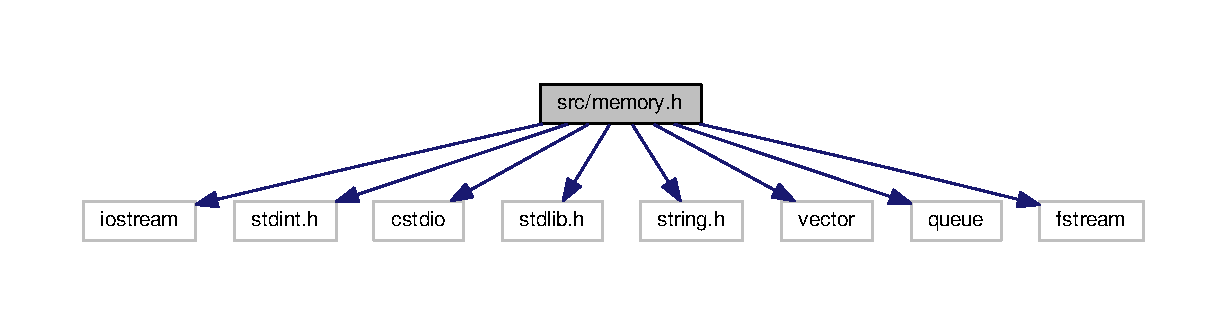
\includegraphics[width=350pt]{memory_8h__incl}
\end{center}
\end{figure}
This graph shows which files directly or indirectly include this file\+:\nopagebreak
\begin{figure}[H]
\begin{center}
\leavevmode
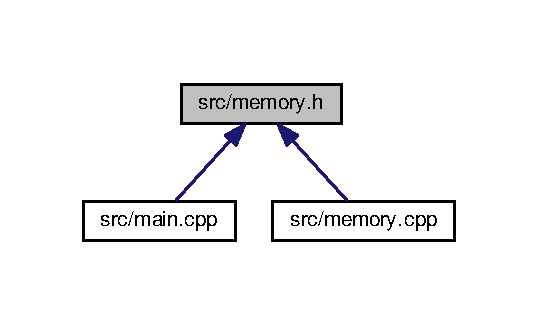
\includegraphics[width=258pt]{memory_8h__dep__incl}
\end{center}
\end{figure}
\subsection*{Classes}
\begin{DoxyCompactItemize}
\item 
class \hyperlink{classPhysicalMemory}{Physical\+Memory}
\begin{DoxyCompactList}\small\item\em Imitates a physical memory. \end{DoxyCompactList}\item 
class \hyperlink{classPageTable}{Page\+Table}
\begin{DoxyCompactList}\small\item\em Page table holding page/frame pairs. \end{DoxyCompactList}\item 
struct \hyperlink{structMemoryPairAddress__t}{Memory\+Pair\+Address\+\_\+t}
\item 
struct \hyperlink{structTLBReturnData__t}{T\+L\+B\+Return\+Data\+\_\+t}
\item 
class \hyperlink{classTranslationLookasideBuffer}{Translation\+Lookaside\+Buffer}
\item 
class \hyperlink{classMemoryManager}{Memory\+Manager}
\begin{DoxyCompactList}\small\item\em A memory management unit. \end{DoxyCompactList}\end{DoxyCompactItemize}
\subsection*{Macros}
\begin{DoxyCompactItemize}
\item 
\#define \hyperlink{memory_8h_af6463c112a252cbb29636eef8ae9e6dc}{E\+N\+A\+B\+L\+E\+\_\+\+L\+RU}
\item 
\#define \hyperlink{memory_8h_af9b1b2ba12857a4bf11289dac8c5462d}{F\+R\+A\+M\+E\+\_\+\+S\+I\+ZE}~256
\item 
\#define \hyperlink{memory_8h_a7d467c1d283fdfa1f2081ba1e0d01b6e}{P\+A\+G\+E\+\_\+\+S\+I\+ZE}~256
\item 
\#define \hyperlink{memory_8h_a0b0ce802de0cae773522024d7626b007}{N\+\_\+\+F\+R\+A\+M\+ES}~8
\item 
\#define \hyperlink{memory_8h_a6fc2e8cefe03a42d0a238bad856a2a8b}{P\+A\+G\+E\+\_\+\+T\+A\+B\+L\+E\+\_\+\+E\+N\+T\+R\+I\+ES}~16
\item 
\#define \hyperlink{memory_8h_a478707addabe7b0aedaa632b70394d75}{B\+A\+C\+K\+E\+N\+D\+\_\+\+FN}~\char`\"{}B\+A\+C\+K\+I\+N\+G\+\_\+\+S\+T\+O\+R\+E.\+bin\char`\"{}
\item 
\#define \hyperlink{memory_8h_a502fddf4e42292e4318a924b6b3b7759}{B\+A\+C\+K\+E\+N\+D\+\_\+\+F\+N\+\_\+\+C\+H\+A\+RS}~18
\item 
\#define \hyperlink{memory_8h_a391c8595be4da3b3f1cd95918b89da2c}{V\+I\+R\+T\+U\+A\+L\+\_\+\+A\+D\+D\+R\+E\+S\+S\+\_\+\+M\+AX}~4095
\item 
\#define \hyperlink{memory_8h_a49009cc208379999b117ed68da61c759}{T\+L\+B\+\_\+\+E\+N\+T\+R\+I\+ES}~4
\end{DoxyCompactItemize}
\subsection*{Functions}
\begin{DoxyCompactItemize}
\item 
\hyperlink{structMemoryPairAddress__t}{Memory\+Pair\+Address\+\_\+t} \hyperlink{memory_8h_a90bdb77a86b4a78c22b50e250b77d9ad}{Convert\+Address\+Format} (int addr)
\begin{DoxyCompactList}\small\item\em Convert a base-\/10 address to (P, d) format. \end{DoxyCompactList}\item 
void \hyperlink{memory_8h_ac93b824d9e950d90189b96ba89151512}{Print\+Memory\+Pair\+Address} (\hyperlink{structMemoryPairAddress__t}{Memory\+Pair\+Address\+\_\+t} mempair)
\end{DoxyCompactItemize}


\subsection{Macro Definition Documentation}
\index{memory.\+h@{memory.\+h}!B\+A\+C\+K\+E\+N\+D\+\_\+\+FN@{B\+A\+C\+K\+E\+N\+D\+\_\+\+FN}}
\index{B\+A\+C\+K\+E\+N\+D\+\_\+\+FN@{B\+A\+C\+K\+E\+N\+D\+\_\+\+FN}!memory.\+h@{memory.\+h}}
\subsubsection[{\texorpdfstring{B\+A\+C\+K\+E\+N\+D\+\_\+\+FN}{BACKEND_FN}}]{\setlength{\rightskip}{0pt plus 5cm}\#define B\+A\+C\+K\+E\+N\+D\+\_\+\+FN~\char`\"{}B\+A\+C\+K\+I\+N\+G\+\_\+\+S\+T\+O\+R\+E.\+bin\char`\"{}}\hypertarget{memory_8h_a478707addabe7b0aedaa632b70394d75}{}\label{memory_8h_a478707addabe7b0aedaa632b70394d75}


Definition at line \hyperlink{memory_8h_source_l00021}{21} of file \hyperlink{memory_8h_source}{memory.\+h}.

\index{memory.\+h@{memory.\+h}!B\+A\+C\+K\+E\+N\+D\+\_\+\+F\+N\+\_\+\+C\+H\+A\+RS@{B\+A\+C\+K\+E\+N\+D\+\_\+\+F\+N\+\_\+\+C\+H\+A\+RS}}
\index{B\+A\+C\+K\+E\+N\+D\+\_\+\+F\+N\+\_\+\+C\+H\+A\+RS@{B\+A\+C\+K\+E\+N\+D\+\_\+\+F\+N\+\_\+\+C\+H\+A\+RS}!memory.\+h@{memory.\+h}}
\subsubsection[{\texorpdfstring{B\+A\+C\+K\+E\+N\+D\+\_\+\+F\+N\+\_\+\+C\+H\+A\+RS}{BACKEND_FN_CHARS}}]{\setlength{\rightskip}{0pt plus 5cm}\#define B\+A\+C\+K\+E\+N\+D\+\_\+\+F\+N\+\_\+\+C\+H\+A\+RS~18}\hypertarget{memory_8h_a502fddf4e42292e4318a924b6b3b7759}{}\label{memory_8h_a502fddf4e42292e4318a924b6b3b7759}


Definition at line \hyperlink{memory_8h_source_l00022}{22} of file \hyperlink{memory_8h_source}{memory.\+h}.

\index{memory.\+h@{memory.\+h}!E\+N\+A\+B\+L\+E\+\_\+\+L\+RU@{E\+N\+A\+B\+L\+E\+\_\+\+L\+RU}}
\index{E\+N\+A\+B\+L\+E\+\_\+\+L\+RU@{E\+N\+A\+B\+L\+E\+\_\+\+L\+RU}!memory.\+h@{memory.\+h}}
\subsubsection[{\texorpdfstring{E\+N\+A\+B\+L\+E\+\_\+\+L\+RU}{ENABLE_LRU}}]{\setlength{\rightskip}{0pt plus 5cm}\#define E\+N\+A\+B\+L\+E\+\_\+\+L\+RU}\hypertarget{memory_8h_af6463c112a252cbb29636eef8ae9e6dc}{}\label{memory_8h_af6463c112a252cbb29636eef8ae9e6dc}


Definition at line \hyperlink{memory_8h_source_l00014}{14} of file \hyperlink{memory_8h_source}{memory.\+h}.

\index{memory.\+h@{memory.\+h}!F\+R\+A\+M\+E\+\_\+\+S\+I\+ZE@{F\+R\+A\+M\+E\+\_\+\+S\+I\+ZE}}
\index{F\+R\+A\+M\+E\+\_\+\+S\+I\+ZE@{F\+R\+A\+M\+E\+\_\+\+S\+I\+ZE}!memory.\+h@{memory.\+h}}
\subsubsection[{\texorpdfstring{F\+R\+A\+M\+E\+\_\+\+S\+I\+ZE}{FRAME_SIZE}}]{\setlength{\rightskip}{0pt plus 5cm}\#define F\+R\+A\+M\+E\+\_\+\+S\+I\+ZE~256}\hypertarget{memory_8h_af9b1b2ba12857a4bf11289dac8c5462d}{}\label{memory_8h_af9b1b2ba12857a4bf11289dac8c5462d}


Definition at line \hyperlink{memory_8h_source_l00015}{15} of file \hyperlink{memory_8h_source}{memory.\+h}.

\index{memory.\+h@{memory.\+h}!N\+\_\+\+F\+R\+A\+M\+ES@{N\+\_\+\+F\+R\+A\+M\+ES}}
\index{N\+\_\+\+F\+R\+A\+M\+ES@{N\+\_\+\+F\+R\+A\+M\+ES}!memory.\+h@{memory.\+h}}
\subsubsection[{\texorpdfstring{N\+\_\+\+F\+R\+A\+M\+ES}{N_FRAMES}}]{\setlength{\rightskip}{0pt plus 5cm}\#define N\+\_\+\+F\+R\+A\+M\+ES~8}\hypertarget{memory_8h_a0b0ce802de0cae773522024d7626b007}{}\label{memory_8h_a0b0ce802de0cae773522024d7626b007}


Definition at line \hyperlink{memory_8h_source_l00017}{17} of file \hyperlink{memory_8h_source}{memory.\+h}.

\index{memory.\+h@{memory.\+h}!P\+A\+G\+E\+\_\+\+S\+I\+ZE@{P\+A\+G\+E\+\_\+\+S\+I\+ZE}}
\index{P\+A\+G\+E\+\_\+\+S\+I\+ZE@{P\+A\+G\+E\+\_\+\+S\+I\+ZE}!memory.\+h@{memory.\+h}}
\subsubsection[{\texorpdfstring{P\+A\+G\+E\+\_\+\+S\+I\+ZE}{PAGE_SIZE}}]{\setlength{\rightskip}{0pt plus 5cm}\#define P\+A\+G\+E\+\_\+\+S\+I\+ZE~256}\hypertarget{memory_8h_a7d467c1d283fdfa1f2081ba1e0d01b6e}{}\label{memory_8h_a7d467c1d283fdfa1f2081ba1e0d01b6e}


Definition at line \hyperlink{memory_8h_source_l00016}{16} of file \hyperlink{memory_8h_source}{memory.\+h}.

\index{memory.\+h@{memory.\+h}!P\+A\+G\+E\+\_\+\+T\+A\+B\+L\+E\+\_\+\+E\+N\+T\+R\+I\+ES@{P\+A\+G\+E\+\_\+\+T\+A\+B\+L\+E\+\_\+\+E\+N\+T\+R\+I\+ES}}
\index{P\+A\+G\+E\+\_\+\+T\+A\+B\+L\+E\+\_\+\+E\+N\+T\+R\+I\+ES@{P\+A\+G\+E\+\_\+\+T\+A\+B\+L\+E\+\_\+\+E\+N\+T\+R\+I\+ES}!memory.\+h@{memory.\+h}}
\subsubsection[{\texorpdfstring{P\+A\+G\+E\+\_\+\+T\+A\+B\+L\+E\+\_\+\+E\+N\+T\+R\+I\+ES}{PAGE_TABLE_ENTRIES}}]{\setlength{\rightskip}{0pt plus 5cm}\#define P\+A\+G\+E\+\_\+\+T\+A\+B\+L\+E\+\_\+\+E\+N\+T\+R\+I\+ES~16}\hypertarget{memory_8h_a6fc2e8cefe03a42d0a238bad856a2a8b}{}\label{memory_8h_a6fc2e8cefe03a42d0a238bad856a2a8b}


Definition at line \hyperlink{memory_8h_source_l00019}{19} of file \hyperlink{memory_8h_source}{memory.\+h}.

\index{memory.\+h@{memory.\+h}!T\+L\+B\+\_\+\+E\+N\+T\+R\+I\+ES@{T\+L\+B\+\_\+\+E\+N\+T\+R\+I\+ES}}
\index{T\+L\+B\+\_\+\+E\+N\+T\+R\+I\+ES@{T\+L\+B\+\_\+\+E\+N\+T\+R\+I\+ES}!memory.\+h@{memory.\+h}}
\subsubsection[{\texorpdfstring{T\+L\+B\+\_\+\+E\+N\+T\+R\+I\+ES}{TLB_ENTRIES}}]{\setlength{\rightskip}{0pt plus 5cm}\#define T\+L\+B\+\_\+\+E\+N\+T\+R\+I\+ES~4}\hypertarget{memory_8h_a49009cc208379999b117ed68da61c759}{}\label{memory_8h_a49009cc208379999b117ed68da61c759}


Definition at line \hyperlink{memory_8h_source_l00026}{26} of file \hyperlink{memory_8h_source}{memory.\+h}.

\index{memory.\+h@{memory.\+h}!V\+I\+R\+T\+U\+A\+L\+\_\+\+A\+D\+D\+R\+E\+S\+S\+\_\+\+M\+AX@{V\+I\+R\+T\+U\+A\+L\+\_\+\+A\+D\+D\+R\+E\+S\+S\+\_\+\+M\+AX}}
\index{V\+I\+R\+T\+U\+A\+L\+\_\+\+A\+D\+D\+R\+E\+S\+S\+\_\+\+M\+AX@{V\+I\+R\+T\+U\+A\+L\+\_\+\+A\+D\+D\+R\+E\+S\+S\+\_\+\+M\+AX}!memory.\+h@{memory.\+h}}
\subsubsection[{\texorpdfstring{V\+I\+R\+T\+U\+A\+L\+\_\+\+A\+D\+D\+R\+E\+S\+S\+\_\+\+M\+AX}{VIRTUAL_ADDRESS_MAX}}]{\setlength{\rightskip}{0pt plus 5cm}\#define V\+I\+R\+T\+U\+A\+L\+\_\+\+A\+D\+D\+R\+E\+S\+S\+\_\+\+M\+AX~4095}\hypertarget{memory_8h_a391c8595be4da3b3f1cd95918b89da2c}{}\label{memory_8h_a391c8595be4da3b3f1cd95918b89da2c}


Definition at line \hyperlink{memory_8h_source_l00024}{24} of file \hyperlink{memory_8h_source}{memory.\+h}.



\subsection{Function Documentation}
\index{memory.\+h@{memory.\+h}!Convert\+Address\+Format@{Convert\+Address\+Format}}
\index{Convert\+Address\+Format@{Convert\+Address\+Format}!memory.\+h@{memory.\+h}}
\subsubsection[{\texorpdfstring{Convert\+Address\+Format(int addr)}{ConvertAddressFormat(int addr)}}]{\setlength{\rightskip}{0pt plus 5cm}{\bf Memory\+Pair\+Address\+\_\+t} Convert\+Address\+Format (
\begin{DoxyParamCaption}
\item[{int}]{addr}
\end{DoxyParamCaption}
)}\hypertarget{memory_8h_a90bdb77a86b4a78c22b50e250b77d9ad}{}\label{memory_8h_a90bdb77a86b4a78c22b50e250b77d9ad}


Convert a base-\/10 address to (P, d) format. 


\begin{DoxyParams}{Parameters}
{\em int} & base-\/10 address to translate \\
\hline
\end{DoxyParams}

\begin{DoxyRetVals}{Return values}
{\em \hyperlink{structMemoryPairAddress__t}{Memory\+Pair\+Address\+\_\+t}} & (P, d) pair corresponding to the address \\
\hline
\end{DoxyRetVals}


Definition at line \hyperlink{memory_8cpp_source_l00457}{457} of file \hyperlink{memory_8cpp_source}{memory.\+cpp}.

\index{memory.\+h@{memory.\+h}!Print\+Memory\+Pair\+Address@{Print\+Memory\+Pair\+Address}}
\index{Print\+Memory\+Pair\+Address@{Print\+Memory\+Pair\+Address}!memory.\+h@{memory.\+h}}
\subsubsection[{\texorpdfstring{Print\+Memory\+Pair\+Address(\+Memory\+Pair\+Address\+\_\+t mempair)}{PrintMemoryPairAddress(MemoryPairAddress_t mempair)}}]{\setlength{\rightskip}{0pt plus 5cm}void Print\+Memory\+Pair\+Address (
\begin{DoxyParamCaption}
\item[{{\bf Memory\+Pair\+Address\+\_\+t}}]{mempair}
\end{DoxyParamCaption}
)}\hypertarget{memory_8h_ac93b824d9e950d90189b96ba89151512}{}\label{memory_8h_ac93b824d9e950d90189b96ba89151512}


Definition at line \hyperlink{memory_8cpp_source_l00465}{465} of file \hyperlink{memory_8cpp_source}{memory.\+cpp}.


\hypertarget{memory_8h_source}{}\section{memory.\+h}
\label{memory_8h_source}\index{src/memory.\+h@{src/memory.\+h}}

\begin{DoxyCode}
00001 \textcolor{preprocessor}{#ifndef \_\_MEMORY\_H\_}
00002 \textcolor{preprocessor}{#define \_\_MEMORY\_H\_}
00003 
00004 \textcolor{preprocessor}{#include <iostream>}
00005 \textcolor{preprocessor}{#include <stdint.h>}
00006 \textcolor{preprocessor}{#include <cstdio>}
00007 \textcolor{preprocessor}{#include <stdlib.h>}
00008 \textcolor{preprocessor}{#include <string.h>}
00009 \textcolor{preprocessor}{#include <vector>}
00010 \textcolor{preprocessor}{#include <queue>}
00011 \textcolor{preprocessor}{#include <fstream>}
00012 \textcolor{keyword}{using namespace }\hyperlink{namespacestd}{std};
00013 
\hypertarget{memory_8h_source.tex_l00014}{}\hyperlink{memory_8h_af6463c112a252cbb29636eef8ae9e6dc}{00014} \textcolor{preprocessor}{#define ENABLE\_LRU}
\hypertarget{memory_8h_source.tex_l00015}{}\hyperlink{memory_8h_af9b1b2ba12857a4bf11289dac8c5462d}{00015} \textcolor{preprocessor}{#define FRAME\_SIZE 256}
\hypertarget{memory_8h_source.tex_l00016}{}\hyperlink{memory_8h_a7d467c1d283fdfa1f2081ba1e0d01b6e}{00016} \textcolor{preprocessor}{#define PAGE\_SIZE 256}
\hypertarget{memory_8h_source.tex_l00017}{}\hyperlink{memory_8h_a0b0ce802de0cae773522024d7626b007}{00017} \textcolor{preprocessor}{#define N\_FRAMES 8}
00018 
\hypertarget{memory_8h_source.tex_l00019}{}\hyperlink{memory_8h_a6fc2e8cefe03a42d0a238bad856a2a8b}{00019} \textcolor{preprocessor}{#define PAGE\_TABLE\_ENTRIES 16}
00020 
\hypertarget{memory_8h_source.tex_l00021}{}\hyperlink{memory_8h_a478707addabe7b0aedaa632b70394d75}{00021} \textcolor{preprocessor}{#define BACKEND\_FN "BACKING\_STORE.bin"}
\hypertarget{memory_8h_source.tex_l00022}{}\hyperlink{memory_8h_a502fddf4e42292e4318a924b6b3b7759}{00022} \textcolor{preprocessor}{#define BACKEND\_FN\_CHARS 18}
00023 
\hypertarget{memory_8h_source.tex_l00024}{}\hyperlink{memory_8h_a391c8595be4da3b3f1cd95918b89da2c}{00024} \textcolor{preprocessor}{#define VIRTUAL\_ADDRESS\_MAX 4095}
00025 
\hypertarget{memory_8h_source.tex_l00026}{}\hyperlink{memory_8h_a49009cc208379999b117ed68da61c759}{00026} \textcolor{preprocessor}{#define TLB\_ENTRIES 4}
00027 
00028 
00029 \textcolor{comment}{// Forward Declarations}
00030 
00031 \textcolor{keyword}{class }\hyperlink{classPhysicalMemory}{PhysicalMemory};
00032 \textcolor{keyword}{class }\hyperlink{classPageTable}{PageTable};
00033 \textcolor{keyword}{class }\hyperlink{classTranslationLookasideBuffer}{TranslationLookasideBuffer};
00034 \textcolor{keyword}{class }\hyperlink{classMemoryManager}{MemoryManager};
00035 
00036 
\hypertarget{memory_8h_source.tex_l00041}{}\hyperlink{classPhysicalMemory}{00041} \textcolor{keyword}{class }\hyperlink{classPhysicalMemory}{PhysicalMemory} \{
00042 
00043 \textcolor{keyword}{public}:
00047     \hyperlink{classPhysicalMemory}{PhysicalMemory}();
00048     
00053     \textcolor{keywordtype}{int} FindFirstFrame();
00054     
00062     \textcolor{keywordtype}{char} GetMemoryContents(\textcolor{keywordtype}{int} frame, \textcolor{keywordtype}{int} offset);
00063 
00068     \textcolor{keywordtype}{bool} isFull();
00069 
00076     \textcolor{keywordtype}{void} PageIn(\textcolor{keywordtype}{int} frame, \textcolor{keywordtype}{char} pagein[\hyperlink{memory_8h_af9b1b2ba12857a4bf11289dac8c5462d}{FRAME\_SIZE}]);
00077 
00083     \textcolor{keywordtype}{void} PageOut(\textcolor{keywordtype}{int} frame);
00084 
00085 \textcolor{keyword}{private}:
00086     \textcolor{keyword}{static} \textcolor{keyword}{const} \textcolor{keywordtype}{int} n\_frames = \hyperlink{memory_8h_a0b0ce802de0cae773522024d7626b007}{N\_FRAMES};
00087     \textcolor{keyword}{static} \textcolor{keyword}{const} \textcolor{keywordtype}{int} frame\_size = \hyperlink{memory_8h_af9b1b2ba12857a4bf11289dac8c5462d}{FRAME\_SIZE};
00088 
00089     \textcolor{keywordtype}{char} memory[n\_frames][frame\_size];
00090 
00094     \textcolor{keywordtype}{char} occupied[n\_frames];
00095 
00096 \};  
00097 
\hypertarget{memory_8h_source.tex_l00102}{}\hyperlink{classPageTable}{00102} \textcolor{keyword}{class }\hyperlink{classPageTable}{PageTable} \{
00103 
00104 \textcolor{keyword}{public}:
00105 
00109     \hyperlink{classPageTable}{PageTable}();
00110 
00116     \textcolor{keywordtype}{int} LookupPage(\textcolor{keywordtype}{int} pagenum);
00117 
00123     \textcolor{keywordtype}{int} LookupPage\_no\_LRU(\textcolor{keywordtype}{int} pagenum);
00127     \textcolor{keywordtype}{void} SetPageToFrame(\textcolor{keywordtype}{int} pagenum, \textcolor{keywordtype}{int} framenum);
00128 
00134     \textcolor{keywordtype}{bool} PageIsValid(\textcolor{keywordtype}{int} pagenum);
00135 
00139     \textcolor{keywordtype}{void} PrintPageTable();
00140 
00144     \textcolor{keywordtype}{void} PrintInversePageTable();
00145 
00151     \textcolor{keywordtype}{int} GetLRUPage();
00152 
00157     \textcolor{keywordtype}{void} UpdateLRUList(\textcolor{keywordtype}{int} last\_used);
00158     
00165     \textcolor{keywordtype}{void} PageOut\_table(\textcolor{keywordtype}{int} pagenum);
00166 
00167 \textcolor{keyword}{private}:
00168     \textcolor{keyword}{static} \textcolor{keyword}{const} \textcolor{keywordtype}{int} pgtable\_entries = \hyperlink{memory_8h_a6fc2e8cefe03a42d0a238bad856a2a8b}{PAGE\_TABLE\_ENTRIES};
00172     \textcolor{keywordtype}{int} pgtable[\hyperlink{memory_8h_a6fc2e8cefe03a42d0a238bad856a2a8b}{PAGE\_TABLE\_ENTRIES}];
00173     \textcolor{keywordtype}{int} valid[\hyperlink{memory_8h_a6fc2e8cefe03a42d0a238bad856a2a8b}{PAGE\_TABLE\_ENTRIES}];
00174     std::vector<int> LRU\_list;
00175 \};
00176 
\hypertarget{memory_8h_source.tex_l00181}{}\hyperlink{structMemoryPairAddress__t}{00181} \textcolor{keyword}{typedef} \textcolor{keyword}{struct }\{
\hypertarget{memory_8h_source.tex_l00182}{}\hyperlink{structMemoryPairAddress__t_a5bc11426b27565b959f280dd1a18b080}{00182}     \textcolor{keywordtype}{int} \hyperlink{structMemoryPairAddress__t_a5bc11426b27565b959f280dd1a18b080}{P};
\hypertarget{memory_8h_source.tex_l00183}{}\hyperlink{structMemoryPairAddress__t_ad608e86288286889c2658e8043414edf}{00183}     \textcolor{keywordtype}{int} \hyperlink{structMemoryPairAddress__t_ad608e86288286889c2658e8043414edf}{d};
00184 \} \hyperlink{structMemoryPairAddress__t}{MemoryPairAddress\_t};
00185 
00191 \hyperlink{structMemoryPairAddress__t}{MemoryPairAddress\_t} \hyperlink{memory_8h_a90bdb77a86b4a78c22b50e250b77d9ad}{ConvertAddressFormat}(\textcolor{keywordtype}{int} addr);
00192 \textcolor{keywordtype}{void} \hyperlink{memory_8h_ac93b824d9e950d90189b96ba89151512}{PrintMemoryPairAddress}(\hyperlink{structMemoryPairAddress__t}{MemoryPairAddress\_t} mempair);
00193 \textcolor{comment}{/*}
00194 \textcolor{comment}{    @class TranslationLookasideBuffer}
00195 \textcolor{comment}{    @brief A TLB used as a cache for memory}
00196 \textcolor{comment}{*/}
00197 
\hypertarget{memory_8h_source.tex_l00198}{}\hyperlink{structTLBReturnData__t}{00198} \textcolor{keyword}{typedef} \textcolor{keyword}{struct }\{
\hypertarget{memory_8h_source.tex_l00199}{}\hyperlink{structTLBReturnData__t_ac4bdfa0ee74b50048e94321426877439}{00199}     \textcolor{keywordtype}{int} \hyperlink{structTLBReturnData__t_ac4bdfa0ee74b50048e94321426877439}{frame};
\hypertarget{memory_8h_source.tex_l00200}{}\hyperlink{structTLBReturnData__t_a58914c8a985e6cdb2f48a56ab41a6985}{00200}     \textcolor{keywordtype}{int} \hyperlink{structTLBReturnData__t_a58914c8a985e6cdb2f48a56ab41a6985}{entry};
00201 \} \hyperlink{structTLBReturnData__t}{TLBReturnData\_t};
00202 
\hypertarget{memory_8h_source.tex_l00203}{}\hyperlink{classTranslationLookasideBuffer}{00203} \textcolor{keyword}{class }\hyperlink{classTranslationLookasideBuffer}{TranslationLookasideBuffer} \{
00204 
00205 \textcolor{keyword}{public}:
00209     \hyperlink{classTranslationLookasideBuffer}{TranslationLookasideBuffer}();
00210 
00215     \textcolor{keywordtype}{bool} isFull();
00216 
00221     \hyperlink{structTLBReturnData__t}{TLBReturnData\_t} LookupTLBFrame(\textcolor{keywordtype}{int} pagenum);
00222 
00230     \textcolor{keywordtype}{int} UpdateTLB(\textcolor{keywordtype}{int} pagenum, \textcolor{keywordtype}{int} framenum);
00231 
00235     \textcolor{keywordtype}{void} PrintTLB();
00236 \textcolor{keyword}{private}:
00237     \textcolor{keywordtype}{int} pagecol[\hyperlink{memory_8h_a49009cc208379999b117ed68da61c759}{TLB\_ENTRIES}];
00238     \textcolor{keywordtype}{int} framecol[\hyperlink{memory_8h_a49009cc208379999b117ed68da61c759}{TLB\_ENTRIES}];
00239     \textcolor{keywordtype}{int} occupied[\hyperlink{memory_8h_a49009cc208379999b117ed68da61c759}{TLB\_ENTRIES}];
00240 
00244     std::queue<int> FIFO\_tlb;
00245 \};
00246 
\hypertarget{memory_8h_source.tex_l00251}{}\hyperlink{classMemoryManager}{00251} \textcolor{keyword}{class }\hyperlink{classMemoryManager}{MemoryManager} \{
00252 \textcolor{keyword}{public}:
00257     \hyperlink{classMemoryManager}{MemoryManager}();
00258     
00265     \textcolor{keywordtype}{char} ReadMemory(\textcolor{keywordtype}{int} addr);
00266 
00273     \textcolor{keywordtype}{int} TranslateAddress(\textcolor{keywordtype}{int} addr);
00274 
00278     \textcolor{keywordtype}{void} PrintPageTable();
00279 
00283     \textcolor{keywordtype}{void} PrintTLB();
00284 
00288     \textcolor{keywordtype}{void} PrintInversePageTable();
00289 
00293     \textcolor{keywordtype}{void} PrintAll();
00294 
00298     \textcolor{keywordtype}{void} PrintStats();
00299 \textcolor{keyword}{private}:
00300     \textcolor{keywordtype}{char}* backend\_store\_filename;
00301 
00302     \hyperlink{classPageTable}{PageTable} page\_table;
00303     \hyperlink{classPhysicalMemory}{PhysicalMemory} physical\_memory;
00304     \hyperlink{classTranslationLookasideBuffer}{TranslationLookasideBuffer} tlb;
00305 
00306     uint32\_t total\_accesses;
00307     uint32\_t page\_faults;
00308     uint32\_t tlb\_hitrate;
00309 
00317     \textcolor{keywordtype}{void} FileSeek(\textcolor{keywordtype}{int} fpage, \textcolor{keywordtype}{char}* dest);
00318 \};
00319 
00320 
00321 \textcolor{preprocessor}{#endif}
\end{DoxyCode}

%--- End generated contents ---

% Index
\backmatter
\newpage
\phantomsection
\clearemptydoublepage
\addcontentsline{toc}{chapter}{Index}
\printindex

\end{document}
